\documentclass[12pt,spanish,oneside]{book}
\usepackage[Algoritmo]{algorithm}
\usepackage{algpseudocode}
\usepackage{epsfig}
\usepackage{epstopdf}
\usepackage[utf8]{inputenc}
\usepackage{pgf,tikz}
\usepackage{pgfplots}
\usetikzlibrary{arrows}
\usepackage{mathrsfs}
\usepackage[spanish,mexico]{babel}
\usepackage{amsmath}
\usepackage{amsfonts}
\usepackage{mathptmx}
\pgfplotsset{compat=1.8}
\usepackage{amssymb}
\usepackage{amsthm}
\usepackage[Sonny]{fncychap} %Sonny, Lenny, Glenn, Conny, Rejne and Bjarne
\usepackage{booktabs}
\usepackage{makeidx}
\usepackage{graphicx}
\usepackage{dsfont}
\usepackage{float}
\theoremstyle{plain}
\newtheorem{teo}{Teorema}[chapter]
\newtheorem{lema}[teo]{Lema}
\newtheorem{prop}[teo]{Proposici\'{o}n}
\newtheorem{algo}[teo]{Algoritmo}
\newtheorem*{cor}{Corolario}
\numberwithin{equation}{chapter}
\theoremstyle{definition}
\usepackage[numbered]{mcode}
\newtheorem{defi}{Definici\'{o}n}[chapter]
\newtheorem{ej}{Ejemplo}[chapter]
\parindent=0in
\theoremstyle{remark}
\newtheorem*{obs}{Observaci\'{o}n}
\newcommand{\re}{\mathbb{R}}
\newcommand{\parc}[2]{\frac{\partial #1}{\partial #2}}
\newcommand{\nat}{\mathbb{N}}
\newcommand{\LD}{\mathcal{L}^2}
\newcommand{\cz}{C_{\scriptscriptstyle{0}}^{\scriptscriptstyle{\infty}}}
\newcommand{\ci}{C^{\scriptscriptstyle{\infty}}}
\newcommand{\icu}{\int_0^1}
\newcommand{\hu}{H^1}
\newcommand{\hcu}{H_0^1}
\newcommand{\intinf}{\int_{-\infty}^{\infty}}
\newcommand{\dxy}{\hspace{5pt} dx\hspace{2pt} dy }
\newcommand{\ds}{\hspace{5pt} ds}
\newcommand{\dx}{\hspace{5pt} dx}
\newcommand{\dxhat}{\hspace{5pt} d\hat{x}_1d\hat{x}_2}
\newcommand{\dxt}{\hspace{5pt} dx_1dx_2}
\newcommand{\intomega}[1]{\iint_\Omega #1 \dxy} %% Para integrar sobre omega, sólo le pones lo que va dentro
\newcommand{\llaves}[1]{\left\lbrace #1\right\rbrace}
\parskip=10pt
\author{Miguel Angel Escalante Serrato}
\title{Revisión e implementación del método de elementos finitos.}
\begin{document}
\definecolor{zzttqq}{rgb}{0,0.4,0.2}
\definecolor{qqqqff}{rgb}{0,0.4,0.2}
\definecolor{ccqqqq}{rgb}{0.8,0,0}
\definecolor{qqwwtt}{rgb}{0,0.4,0.2}
\definecolor{qqtttt}{rgb}{0,0.2,0.2}
\definecolor{mycolor1}{rgb}{0,0.4,0.2}%
\newpage

\thispagestyle{empty}

\setcounter{page}{1}
\begin{center}
\begin{tabular}{c}
\hline
 \large \emph{\textsc{Instituto Tecnológico Autónomo de México}} \\
 
\hline
\end{tabular}

\vspace{10pt}

\centering
\includegraphics[width=0.8\linewidth]{img/Logo_ITAM.jpeg}

\vspace{20pt}


\Large Revisión e implementación del método de elementos finitos.



\vspace{30pt}

\normalsize TESIS

\vspace{12pt}

que para obtener el título de

\vspace{12pt}

Licenciado en Matemáticas Aplicadas

\vspace{12pt}

presenta

\vspace{12pt}

Miguel Angel Escalante Serrato

\vspace{32pt}

\begin{tabular}{lcr}
MÉXICO, D.F. & \hspace{80pt} & 2013
\end{tabular}

\textbf{Asesor:} Juan Carlos Aguilar Villegas

\textbf{Revisor:} José Luis Farah Ibáñez
\end{center}


\newpage
\setcounter{page}{1}
\pagenumbering{roman}
\mbox{ }
\vspace{80pt}
\mbox{ }

Con fundamento en los artículos 21 y 27 de la Ley Federal del Derecho de Autor y como titular de los derechos moral y patrimonial de la obtra titulada ``\textbf{Revisión e implementación del método de elementos finitos.}'', otorgo de manera gratuita y permanente al Instituto Tecnológico Autónomo de México y a la Biblioteca Raúl Bailléres Jr., autorización para que fijen la obra en cualquier medio, incluido el electrónico, y la divulguen entre sus usuarios, profesores, estudiantes o terceras personas, sin que pueda percibir por tal divulgación una contraprestación.
\vspace{20pt}
\begin{center}
\textbf{Miguel Angel Escalante Serrato}
\vspace{80pt}

\begin{tabular}{p{2cm}cp{2cm}}

\hline \\
 

&Fecha & \\
\\
\\
\\
\\
\\
\\
\\
\\
\hline \\

 & Firma & 

\end{tabular}
\end{center}



\newpage
\thispagestyle{empty}

\begin{center}

\vspace{40pt}
\[\]
\[\]
\[\]
\begin{tabular}{c}
\hline
 \\[.2cm]
\Huge
\textbf{Revisión e implementación del }\\ 
\Huge\textbf{método de elementos finitos }\\[14pt]
\normalsize
Miguel Angel Escalante Serrato \\[.2cm]

\hline
\end{tabular}
\end{center}



\newpage
\vspace*{\fill}
\begin{flushright}
A mi Chango, Jefecita y Caranala.
\vfill
\end{flushright}
\newpage
\mbox{ }
\vspace{80pt}
\begin{flushright}
\textsc{\large Agradecimientos} \\
\vspace{12pt}
A mis padres ya que sin ellos, nada de esto pudo haber sucedido. A mi hermana por ser mi compañera incondicional.

A mi asesor Juan Carlos Aguilar por su paciencia y apoyo durante todo este tiempo.

A mis sinodales José Luis Farah, José Luis Morales y Zeferino Parada portomarse el tiempo de leer este documento y por sus valiosas recomendaciones.

Al Animalito Salvaje, por las sesiones cafeteras y correcciones de todo tipo.

Al profesor Morones por sus comentarios desde España.

A mis amigos que de una u otra manera, alentado o ayudado a este trabajo. Rafa, Irving, Stefania, Alfredo, Maite, Andy, Marina, René.

A Anita por todo el apoyo, cariño y tiempo.


\end{flushright}

\chapter*{Prefacio}

Un problema bastante común en diversas áreas científicas es el de resolver ecuaciones diferenciales parciales, es un problema tanto interesante como relevante ya que es muy usado, por ejemplo, en diversas áreas para modelar la reacción de distintos materiales a diversas condiciones y situaciones. Existen diversos métodos para resolver este tipo de ecuaciones; dependiendo del problema se debe de analizar qué herramienta es la más adecuada para el trabajo. Aquellos problemas en donde una malla no es lo suficientemente robusta para describir el dominio, es el tipo de problemas en los que el método de los elementos finitos se especializa. En particular en esta tesis se implementa un método para resolver un subconjunto de la amplia familia de ecuaciones diferenciales parciales, las elípticas. Es un trabajo que nace de la curiosidad de lo que hay más allá de la solución exacta en pizarrón o papel y lápiz; ¿qué pasa cuando el papel y el lápiz no pueden resolver el problema? ¿Qué pasa cuando se tiene que usar el poder de cómputo? Con la guía y apoyo de mi asesor fui respondiendo estas preguntas para este problema y espero sirva para que el lector encuentre una vela para buscar el camino a la respuesta que busca. 

\frontmatter


\tableofcontents

\mainmatter
\chapter{Introducción}

El modelado es una de las herramientas más poderosas de la matemática actual. Muchos modelos en diversas áreas científicas tienen la forma de ecuaciones diferenciales o integrales. La capacidad de cómputo ha crecido considerablemente desde los inicios del cálculo numérico. Gracias a esto es posible modelar y resolver problemas cada vez más grandes y complejos, por lo que la necesidad de métodos eficientes para el cómputo se hace evidente. En este trabajo estudiamos un problema que tiene relevancia en toda clase de problemas físicos: ecuaciones diferenciales parciales. Dentro de las aplicaciones, ingeniería estructural, resistencia de materiales, mecánica de fluidos, ingeniería nuclear, electromagnetismo, propagación de onda, etc.

La resolución de ecuaciones diferenciales parciales es parte de nuestra vida cotidiana aunque no lo veamos explícitamente; se usa en una gran variedad de modelos para diseñar objetos que tenemos hoy en día, desde piezas de autos hasta aparatos más pequeños como los celulares. El Método de Elementos Finitos (MEF) es una herramienta que ayuda a resolver las ecuaciones necesarias.

El MEF es una técnica general que resuelve numéricamente ecuaciones diferenciales parciales; el método que se programó para este trabajo, resuelve ecuaciones diferenciales parciales elípticas, aunque puede ser adaptado para otro tipo de problemas, ecuaciones parabólicas por ejemplo. 

Uno de los primeros antecedentes del MEF, vino con un trabajo en 1909 por W. Ritz donde desarrolla un método de aproximación para problemas de mecánica en sólidos deformables. Más tarde, en 1943 R. Courant expandió el trabajo hecho por Ritz al introducir funciones lineales sobre dominios triangulares, sin embargo el desarrollo se retoma hasta años más tarde; el MEF como se plantea en este trabajo fue desarrollado por ingenieros de la universidad de Berkeley, a finales de los años 50, principios de los años 60, y en particular se generó como una técnica particular para resolver algunos problemas de estructuras en ingeniería. A mediados de los años 60, conforme se estudiaba, fue resultando evidente el hecho que es en realidad una técnica general para resolver ecuaciones diferenciales parciales, esto con base en la teoría variacional planteada a principios de siglo. Conforme fue avanzando el tiempo el MEF fue generalizado de tal manera que resolviese todo tipo de ecuaciones diferenciales e integrales. 

Actualmente el MEF es usado en los programas de Diseño Asistido por Computadora (CAD por sus siglas en inglés). Los CAD pueden simular una gama amplia de condiciones como temperatura, elasticidad, materiales, fuerza aplicada y otros más, haciéndolos una herramienta clave para cualquier diseño

El MEF es un método muy usado por la simplicidad teórica así como la gran cantidad de problemas que puede atacar, todo esto sin demasiada complicación algorítmica, dejando así un método elegante y poderoso. 

A continuación introduciremos ejemplos de los problemas que se pueden resolver con el MEF. 

\begin{ej}
Encontrar $u$ tal que: 
\begin{equation}\label{eq1}
\begin{aligned}
-\Delta u &= f \hspace{10 pt} \text{en } \Omega \subset \re^2, \hspace{5pt} \\
u &=0 \hspace{10 pt} \text{en } \Gamma,
\end{aligned}
\end{equation}
donde \[\Delta u = \frac{\partial^2 u}{\partial x_1^2}+\frac{\partial^2 u}{\partial x_2^2},\] $\Omega $ es el dominio de la función $u$, el cual es abierto y acotado, con frontera $\Gamma$ de clase $C^1$ por trozos. 
\end{ej}
Este es el ejemplo más sencillo y conocido de las ecuaciones diferenciales parciales elípticas y podemos ampliar la ecuación \ref{eq1}, cambiando la condición de frontera y hacerla no homogénea:
\begin{ej}
Encontrar $u$ tal que: 
\begin{align*}
-\Delta u &= f \hspace{10 pt} \text{en } \Omega \subset \re^2, \\
u &=g\hspace{10 pt} \text{en } \Gamma, 
\end{align*}
donde $g$ es una función de clase $ C^1$.
\end{ej} 

Además podemos explorar maneras de resolver ecuaciones con condiciones de frontera más complicadas: 

\begin{ej}\label{otrcond}
Encontrar $u$ tal que: 
\begin{align*}
-\Delta u &= f \hspace{10 pt} \text{en } \Omega \subset \re^2 , \\
u &=g_1 \hspace{10 pt} \text{en } \Gamma_1 , \text{long}(\Gamma_1)>0,\\
\parc{u}{\eta} &=g_2 \hspace{10 pt} \text{en } \Gamma_2 , \Gamma= \Gamma_1\cup \Gamma_2,
\end{align*}

donde $\parc{u}{\eta}$ es la derivada direccional de $u$ en la dirección $\eta$, que es un vector normal unitario a la curva cerrada $\Gamma$ y que apunta hacia ``afuera''.
\end{ej}

Varios métodos para aproximar la solución de estas ecuaciones tienen la misma idea: discretizar reduciendo el problema de encontrar la función $u$, al de encontrar una serie de coeficientes; esto para encontrar una representación de $u$ de tal manera que: 

\[u(x) \approx \sum_{i=1}^n\alpha_i \phi_i(x), \]

donde $\lbrace x_i\rbrace_{i=1}^n$ son los puntos donde nos interesa conocer el valor de la función, $\lbrace \phi_i \rbrace_{i=1}^n$ son funciones base que se usarán para aproximar $u$, $n$ es el tamaño de la base que se usará y finalmente $\alpha_i$ son los coeficientes asociados con las funciones $\phi_i$.

El MEF se caracteriza por la forma en que se particiona el dominio (triángulos o cuadriláteros en el caso de dos dimensiones) y porque el tipo de funciones base que usa son polinomiales por trozos y de soporte compacto.

Se hizo una implementación de este método en MATLAB, resuelve ecuaciones diferenciales parciales no homogéneas, y puede ser extendido a resolver otro tipo de ecuaciones, como parabólicas o con condiciones de frontera como las planteadas en el ejemplo \ref{otrcond}, e inclusive con distintas funciones base, como cuadráticas o cúbicas.

Este trabajo se estructuró de la siguiente manera, en el capítulo 2 mencionaremos algunos conceptos teóricos necesarios para la resolución del problema, el capítulo 3 aborda conceptos más particulares del MEF así como algunas características del mismo, en el capítulo 4 se menciona la implementación del método en una dimensión, con generalizaciones a otros problemas, el capítulo 5 ilustra los resultados del método programado para funciones en dos dimensiones.

 
\chapter{Conceptos} 

En este capítulo, daremos la teoría necesaria para trabajar con el método de elementos finitos. Primero necesitamos retomar algunos conceptos de álgebra lineal y análisis funcional.

\section{Espacios de Hilbert}

\begin{defi}

Un \textit{espacio vectorial} $V$ sobre $\re$ consiste en un conjunto donde están definidas dos operaciones $+:V\times V\rightarrow V$ y $\cdot : V\times \re \rightarrow V$, con las siguientes propiedades:
\begin{itemize}
\item $\forall x,y \in V$ $x+y=y+x.$

\item $\forall x,y,z \in V$ $(x+y)+z=x+(y+z).$

\item Existe un elemento en $V$ llamado 0 tal que $x+0=x$ $\forall x\in V. $

\item $\forall x \in V\phantom{\pi}\exists y $ tal que $x+y=0.$

\item $\forall x \in V$ $1x=x.$

\item $ \forall \alpha ,\beta \in \re ,x\in V$ $ (\alpha \beta )x = \alpha (\beta x) = \beta (\alpha x).$

\item $\forall x,y\in V \alpha \in \re$ $ \alpha (x+y)= \alpha x +\alpha y .$

\item $\forall \alpha ,\beta \in \re ,x\in V$ $ (\alpha+\beta)x =\alpha x+ \beta x.$


\end{itemize}

\end{defi}
\begin{defi}
Sea $H$ un espacio vectorial, decimos que $\left<\cdot,\cdot\right>:H\times H \longrightarrow \re$ es una \textit{forma bilineal } si es lineal en cada componente. Es decir que para todos $\alpha,\beta\in \re, v,w,z\in H$ tenemos lo que sigue: 
\[ \left<\alpha v+ \beta w,z\right>= \alpha\left<v,z\right>+\beta \left<w,z\right>, \]
\[ \left<z,\alpha v+ \beta w\right>= \alpha\left<z,v\right>+\beta \left<z,w\right>. \]
\end{defi}

\begin{defi}
Sea $H$ un espacio vectorial sobre $\re$. Un \textit{producto interior} en $H$ es una forma bilineal $\left<\cdot,\cdot\right>_H:H\times H \longrightarrow \re$ que satisface lo siguiente: 

\begin{enumerate}
\item $\left<u,v\right>_H=\left<v,u\right>_H \hspace{3pt} \forall u,v \in H$ 
\item $\left<v,v\right>_H \hspace{1pt}\geq 0\hspace{3pt} \forall v\in H$
\item $\left<v,v\right>_H =0 \iff v=0$
\end{enumerate}
\end{defi}

Un espacio vectorial con producto interior tiene una norma inducida por ese producto interior, misma que está dada por: 
\[||v||_H=\sqrt{\left<v,v\right>}_H.\]

\begin{teo}{(Desigualdad de Cauchy-Bunyakovsky-Schwarz (CBS))}
La \\siguiente desigualdad se cumple para todo espacio vectorial con norma inducida por el producto interior:
\[| \left<u,v\right>_H |\leq ||u||_H ||v||_H.\]
\end{teo}

\begin{defi}
Sea $H$ un espacio vectorial con norma $||\cdot||_H$. Se dice que una sucesión $\left \lbrace v_i \right \rbrace_{i\in \nat}$ en $ H $, es de \textit{Cauchy}, si se cumple que $||v_i-v_j||_H \rightarrow 0 $ cuando $i,j\rightarrow \infty$.
\end{defi}

\begin{defi}
Un espacio vectorial $H$ con norma $||\cdot||_H$ es \textit{completo} $\iff$ Para cualquier sucesión de Cauchy $\left \lbrace v_i \right \rbrace_{i\in \nat}$ en $ H $, existe $v\in H$ tal que $||v_i-v||_H\rightarrow 0$ cuando $i \rightarrow \infty$. 
\end{defi}
\begin{defi}
Un \textit{espacio de Hilbert} es un espacio vectorial con producto interior y que es completo con respecto a la norma inducida $||\cdot||_H$.

\end{defi}

\begin{defi}

Sea $H$ espacio de Hilbert con producto interior $\left<\cdot,\cdot\right>_H$. Se dice que $u,v\in H$ son \textit{ortogonales} si $\left<u,v\right>_H=0$.

\end{defi}

\begin{teo}{(De la proyección ortogonal para espacios de dimensión finita )}

Si $H$ es un espacio de Hilbert, $ H'\subset H$ un subespacio vectorial de dimensión finita, y si $u\in H$, $w\in H'$ satisfacen que:

\[\left<u - w,v\right>_H=0\hspace{5pt}\forall v\in H',\]
entonces 
\[||u- w||_H\leq ||u-v||_H \hspace{5pt} \forall v \in H'.\]
\end{teo}

El siguiente es un ejemplo de espacio de Hilbert.

Sea $I=[0,1]\subset \re $ y 
\[\LD(I)=\left \lbrace \text{funciones}\hspace{5pt} v:[0,1]\rightarrow \re\hspace{5pt} \middle| \int_0^1|v(x)|^2 \dx < \infty \right \rbrace\footnote{En realidad el espacio $ \LD(I)$ está formado por clases de equivalencia: dos funciones $g_1$ y $g_2$ están en la misma clase de equivalencia si $g_1$ y $g_2$ son iguales excepto posiblemente en un conjunto de medida cero. }. \]
El espacio de funciones $\LD(I)$ con el producto interior dado por: 
\[\left<u,v\right>_{\LD} = \int_0^1 u(x)v(x)\dx\hspace{10pt}\forall u,v\in \LD(I),\]
es un espacio de Hilbert.

En este caso la desigualdad de CBS es:
\[ \left|\left<u,v\right>\right|^2 \leq ||u||_{\LD}^2 ||v||^2_{\LD}, \]
\[\text{donde } ||u||^2_{\LD}=\int_0^1|u(x)|^2\dx.\]

Los siguientes espacios, son interesantes por su relación con $\LD(I)$. 
\[\ci(I)=\left \lbrace \text{funciones } v:[0,1]\rightarrow \re\hspace{5pt} \big|\hspace{5pt} v \text{ tiene derivadas de todos los \'ordenes} \right \rbrace\]
\[\cz(I)=\left \lbrace \text{funciones } v:[0,1]\rightarrow \re\hspace{5pt} \big| \hspace{5pt}v \text{ es de clase } C^\infty\text{ y con soporte }\subset (0,1)\ \right \rbrace\]
El espacio $\cz(I)$ es denso en $\LD(I)$. Lo que quiere decir que \[\forall u \in \LD(I)\text{ y }\varepsilon >0\hspace{5pt}\exists v \in \cz(I)\text{ tal que }||u-v||_{\LD} < \varepsilon.\]
\begin{teo}\label{igualdad}
Si $g_1,g_2\in \LD(I)$ y:
\[\icu g_1(x)v(x)\dx=\icu g_2(x)v(x) \dx \hspace{5pt} \forall v \in \cz(I), \text{ entonces } g_1=g_2. \]
La igualdad $g_1=g_2$ es en el sentido de las funciones en $\LD$ es decir, $g_1\text{ y } g_2 $ difieren en un conjunto de medida cero\footnote{Para mayor referencia al concepto de medida, consultar \cite{grabs}}.
\end{teo}
Para facilidad de prueba, probemos antes el siguiente lema:

\begin{lema}
Si existe $f\in\LD(I)$ tal que:

$$\icu f(x)v(x)\dx=0\hspace{3pt}\forall v\in  C_0^\infty,$$ entonces $f=0.$
\end{lema}
\begin{proof}
Sea $f\in\LD(I)$, tal que \[\icu f(x)v(x)\dx=0\hspace{3pt}\forall v\in  C_0^\infty, \]
$$0\leq ||f||_{\LD}^2=\left|0-\icu f^2(x)\dx\right|=\left|\icu f(x) v(x)\dx-\icu f^2(x)\dx\right|, \hspace{3pt} \forall	v\in  C_0^\infty.$$

Sabemos que el espacio $ C_0^\infty$ es denso en $\LD(I)$ y por lo tanto, para cada $\varepsilon>0$, existe $v_\varepsilon\in  C_0^\infty $ tal que $||f-v_\varepsilon||_{\LD(I)}<\varepsilon,\hspace{3pt} \forall \varepsilon >0.$

Por lo tanto, para cualquier $\varepsilon>0$

$$||f||_{\LD}^2= \left|\icu f(x) v_\varepsilon(x)\dx-\icu f^2(x)\dx\right|=\left|\icu f(x) \left[v_\varepsilon(x)- f(x)\right]\dx\right| $$
$$\leq \icu\left| f(x) \left[v_\varepsilon(x)- f(x)\right]\right|\dx\leq ||f||_{\LD(I)} ||v_\varepsilon -f||_{\LD(I)}$$ 

De lo cual, $||f||_{\LD}\leq ||v_\varepsilon-f||_{\LD}\leq \varepsilon\hspace{3pt}\forall\varepsilon >0$. Por lo tanto, $f=0$.
\end{proof}
\begin{proof}{(del teorema \ref{igualdad})}
Tenemos
\[\icu g_1(x)v(x)\dx=\icu g_2(x)v(x) \dx \hspace{5pt} \forall v \in \cz(I) \]
\[\Rightarrow\icu g_1(x)v(x)\dx-\icu g_2(x)v(x)\dx=0\]
\[\Rightarrow\icu (g_1(x)- g_2(x))v(x)\dx=0\]
\[\Rightarrow g_1-g_2=0\]
\[\Rightarrow g_1=g_2.\]
\end{proof}

\section{Integración por partes}
Recordemos la fórmula de integración por partes de Cálculo:
\[\int_0^1 u(x) v'(x) \hspace{5pt} dx = u(1)v(1)- u(0)v(0) -\int_0^1 v(x)u'(x) \hspace{5pt} dx, \]
con $u$ y $v$ de clase $ C^1$ en $[0,1]$.

Por lo tanto si $u,v:[0,1]\rightarrow \re$ son funciones de clase $ C^1$ y si $v\in\cz(I)$:
\[\icu u(x) v'(x) \dx =-\icu u'(x) v(x) \dx \hspace{5pt} \forall v \in \cz(I). \]
Esto gracias a que $v(0)=v(1)=0$.

\section{Derivada débil de funciones en $\LD(I)$}

Sea $ u\in \LD(I) $ no necesariamente diferenciable. Se dice que $u$ tiene una \textbf{derivada débil} en $\LD(I)$ si existe $g\in \LD(I)$ tal que:
\[\icu u(x) v'(x)\dx=-\icu g(x) v(x) dx, \hspace{5pt} \forall v \in \cz(I).\]
En este caso se dice que $g$ es una derivada débil de $u$. 

Se tiene que si $u$ es de clase $ C^1$, entonces existe la derivada débil de $u$ y además coincide con la derivada tradicional $u'$. Esto porque la derivada débil (si existe) es única, como se muestra en el siguiente resultado.

\begin{teo}{(Unicidad de la derivada débil)}
Sea $u\in \LD(I)$ tal que $u$ tiene una derivada débil en $\LD(I)$. Si $g_1 \text{ y } g_2\in \LD(I)$ son derivadas débiles de $u$, entonces $g_1=g_2$. 
\end{teo}
\begin{proof}
Sean $u\in\LD(I)$, y $ g_1,g_2\in \LD(I)$ derivadas débiles de $u$.
\begin{align*}
\icu u(x) v'(x)\dx=-\icu g_1(x) v(x)\dx & \hspace{4pt}\forall v \ \cz(I),\\
\icu u(x) v'(x)\dx=-\icu g_2(x) v(x)\dx & \hspace{4pt}\forall v \ \cz(I),\\
\Rightarrow\icu g_1(x) v(x)=\icu g_2(x) v(x)\dx &\hspace{4pt} \forall v \ \cz(I),\\
\end{align*}
y por el Teorema \ref{igualdad} tenemos que $g_1=g_2$.
\end{proof}

Si $u\in \LD(I)$ es continua en $[0,1]$ y lineal por trozos, entonces $u$ tiene una derivada débil, la cual es una función constante por trozos. Pero no cualquier función tiene una derivada débil, como se ilustra en el siguiente ejemplo:
Si $u\in \LD(I)$ tiene una discontinuidad de salto, entonces $u$ no tiene derivada débil en $\LD(I)$. Veamos el siguiente ejemplo: 

Sean $a,b\in \re, a\neq b, x_0\in (0,1)$.
\[\text{Sea } u(x)=\left \lbrace \begin{array}{ccc} a &\text{ si } & 0\leq x\leq x_0 \\ b &\text{ si } & x_0< x\leq 1 \end{array}\right. ,\]
Para probar que $u$ no tiene derivada débil en $\LD(I)$, denotemos primero: 
\[u(x_o^+)=\lim_{x\rightarrow x_o^+}u(x)=b ,\]\[ u(x_o^-)=\lim_{x\rightarrow x_o^-}u(x)=a. \]
Ahora tomemos $v\in \cz(I)$ e integremos sobre $I$.
\[\icu u(x)v'(x)\dx=\int_0^{x_0}u(x)v'(x)\dx +\int_{x_0}^1 u(x)v'(x)dx\]
\[=v(x_0^-)u(x_0^-)-v(0)u(0)-\int_0^{x_0}u'(x)v(x)\dx\]
\[+v(1)u(1)-v(x_0^+)u(x_0^+)-\int_{x_0}^1 u'(x)v(x)\dx \]
\[= 0+a v(x_0)-0-0-bv(x_0)+0 \]
\[= (a-b)\cdot v(x_0)\]
\[\therefore \icu u(x)v'(x)=(a-b)\cdot v(x_0),\]
y deberíamos encontrar una $g$ de tal manera que
\[ \icu u(x)v'(x)=-\icu g(x) v(x)\dx =(a-b)\cdot v(x_0), \hspace{3pt} \forall v \in C_0^{\infty} (I). \]
Pero no existe $g \in \LD(I)$ con la propiedad anterior. Un múltiplo de la Delta de Dirac ($(a-b)\cdot \delta_{x_0}$) satisface la propiedad anterior; de hecho $g$ es un múltiplo constante de la Delta de Dirac . Por lo tanto, $u(x)$ no tiene derivada débil en $\LD(I)$. 

Queda demostrar que
\begin{equation}
\delta_{x_0}\notin\mathcal{L}^2(I).\label{deltanotin}
\end{equation}
Pero antes se muestra un resultado más sencillo que ayudará a demostrar lo anterior.

Sea $f\in\LD(I)$ con $||f||_{\LD}=c$, por simplicidad en este caso $I=[-1,1]$. Se tiene que: 
\[\int_{-1}^1|f(x)|^2\dx=c^2,\]sea $\lambda>1$; se define la función 
\begin{equation}
f'_{\lambda}(x)=f(\lambda x),\label{flambda}
\end{equation}
su norma calculada como sigue:
\[||f'_{\lambda}||=\int_{-1}^1|f(\lambda x)|^2\dx \] con el cambio de variable $u=\lambda x, du=\lambda dx$ queda lo siguiente: 
\[\int_{-\lambda}^{\lambda}|f(u)|^2\frac{1}{\lambda} \hspace{5pt} du =\int_{-1}^{1}|f(u)|^2\frac{1}{\lambda} \hspace{5pt} du =  \frac{1}{\lambda}c^2 \]
por lo tanto tenemos que, si definimos ahora la función $f_{\lambda}(x)=\sqrt{\lambda} f(\lambda x)$, $||f_{\lambda}||=||f||=c$.

\begin{proof}
(De (\ref{deltanotin})) Por simplicidad suponemos que $x_0=0$, y que el intervalo sigue siendo $I=[-1,1]$. Para demostrar que delta no pertenece a $\LD(I)$, suponemos lo contrario, \textit{i.e.} $\delta_0\in\LD(I)$, y se llegará a una contradicción.

Sea entonces la función $f\in \ci(I)$, definida como sigue:
\begin{equation} 
f(x)=\left \lbrace \begin{array}{ccc} e^{\frac{-1}{1-x^{2}}} &\text{ si } & |x|<1 \\ 0 & & \text{ en otro caso} \end{array}\right.,\label{fcompact}
\end{equation}
sea $k$ tal que $||f||=k$.

Si $\delta_{0}\in\LD(I)\Rightarrow\exists M\in\re^{+}$ tal que: \[\int_{-1}^1\delta_{x_0}^2(x)\dx=||\delta_{0}||_{\LD}\leq M.\] 
Ahora tomamos la transformación (\ref{flambda}) de la función (\ref{fcompact}) con $\lambda=(M+1)^2e^{2}k^2$. Podemos tomar $M>1$ tal que $\lambda>1$. En este caso $f_{\lambda}\in \cz(I) $, por lo que: 
\[\int_{-1}^1\delta_0f_{\lambda}(x)\dx = f_{\lambda}(0).\]

Sabemos por la desigualdad CBS:
\[\left|\int_{-1}^1 \delta_{0} f_{\lambda}(x)\dx\right|\leq ||\delta_{x_0}||_{\mathcal{L}^2}||f_{\lambda}||_{\mathcal{L}^2} \]
\[\Rightarrow |f_{\lambda}(0)| \leq ||\delta_{0}||_{\LD}k \]
\[\Rightarrow |\sqrt{\lambda}e^{-1}| \leq ||\delta_{0}||_{\LD}k \]
\[\Rightarrow (M+1)ke^{-1}e^{1}\leq ||\delta_{0}||_{\LD} k \]
\[\Rightarrow (M+1)\leq M. \]
Por ende se concluye que $\delta_0$ no puede pertenecer a $\LD(I)$.
\end{proof}

\section{Derivada débil en $\LD(\Omega)$}

Sea $u\in\LD(\Omega),(u=u(x_1,x_2))$, se dice que $g\in\LD(\Omega)$ es una derivada débil de $u$ con respecto a la variable $x_i$ si:
\[\intomega{u \parc{v}{x_i}}=-\intomega {g v}\hspace{4pt} \forall v\in \cz(\Omega).\]
Se puede probar de forma similar al caso univariado, que si $u$ tiene derivada débil respecto a $x_i$, entonces la derivada débil es única.

\section{Espacios $\LD(\Omega),\hu(\Omega),\hcu(\Omega)$}

Sea $\Omega$ un subconjunto abierto y acotado de $\re^2$. Los siguientes son ejemplos de espacios de Hilbert.
\begin{enumerate}
\item[a)] $\LD(\Omega)=\left \lbrace v:\Omega\rightarrow \re \hspace{5pt} \middle| \displaystyle\iint_\Omega v^2\dxy<\infty\right \rbrace$.

El producto interior y norma que asignamos a este espacio son:
\[\left<u,v\right>_{\LD}=\displaystyle\iint_\Omega u v\dxy,\]
\[||v||^2_{\LD}=\iint_\Omega	v^2\dxy.\]
\item[b)] $\hu (\Omega)= \left \lbrace v \in \LD(\Omega) \hspace{5pt}\middle|\hspace{5pt} \displaystyle\parc{v}{x},\parc{v}{y} \in \LD(\Omega) \right \rbrace$.

Las derivadas referidas en este espacio son en el sentido de las derivadas débiles. El producto interior y norma que asignamos son:
\[ \left<u,v\right>_{\hu}=\intomega{\left(uv + \nabla u \cdot \nabla v\right)},\]
\[||v||^2_{\hu}=\intomega{\left(v^2 + \nabla v \cdot \nabla v\right)}=\intomega{\left(v^2 + |\nabla v|^2\right)}.\]
El espacio $\hu$ contiene las funciones continuas y lineales por trozos.
\item[c)] $\hcu(\Omega) = \left\lbrace v \in \hu(\Omega) \hspace{5pt}\middle|\hspace{5pt} \displaystyle\parc{v}{x},\parc{v}{y} \in \LD(\Omega),v=0 \text{ sobre } \Gamma=\partial\Omega\right \rbrace.$

El producto interior y norma que asignamos a este espacio son los mismos que tenemos para $\hu(\Omega)$. 
\end{enumerate}


\section{Formulación variacional}

Un problema variacional es un problema que optimiza sobre funcionales continuos\footnote{Para mayor referencia a análisis funcional y a problemas variacionales, revisar \cite{funcional1} y \cite{funcional2}} definidos sobre un espacio funcional.
Resolver una ecuación diferencial del estilo: 
\begin{align}\label{1.11}
-\Delta u &= f \hspace{10 pt} \text{en } \Omega \subset \re^2 , \\
u &=0 \hspace{10 pt} \text{en } \Gamma=\partial\Omega.\nonumber
\end{align}
Es equivalente a resolver el siguiente problema variacional.

Encontrar $u\in \hcu(\Omega)$ tal que:
\begin{align}
a(u,v)=\left<f,v\right> \forall v\in \hcu(\Omega),\label{1.3}
\end{align}
donde
\begin{equation*}
a(u,v)=\iint_\Omega \nabla u\cdot \nabla v \dxy =\iint_\Omega \parc{u}{x} \frac{\partial v}{\partial x}+\frac{\partial u}{\partial y} \frac{\partial v}{\partial y} \dxy,
\end{equation*}
y 
\begin{equation*}
\left<f,v\right>=\iint_\Omega f v\dxy.
\end{equation*}

Para probar esta equivalencia entre nuestros problemas, enunciaremos el teorema de la divergencia.

\begin{teo}{(De la Divergencia\footnote{Para mayor referencia ver \cite{Apostol}.})} Sea $A:\Omega \rightarrow \re^2$ una función con valores vectoriales $A=(A_1,A_2)$ y sea $\eta=(\eta_1,\eta_2)$ el vector unitario perpendicular a la curva $\Gamma$ (frontera de $\Omega$) que apunta ``hacia afuera". Entonces tenemos:
\begin{equation}
\iint_{\Omega} div(A) \dxy = \int_{\Gamma} A\cdot \eta \ds.
\end{equation}
Donde $div(A)$ denota la divergencia de la función $A$ y se define como sigue.
\[div(A) = \frac{\partial A_1}{\partial x_1}+\frac{\partial A_2}{\partial x_2}.\]
\end{teo}

Con el teorema de la divergencia deduciremos una fórmula de Green.

Sean $v,w:\Omega \rightarrow \re$, $v$ de clase $ C^1$, $w$ de clase $ C^2$, y sean $A_\alpha,A_\beta:\Omega\rightarrow \re^2$ definidas como sigue: $ A_\alpha=(vw,0),A_\beta=(0,vw) $. 
Sabemos que: 
\[ div(A_\alpha)= \frac{\partial v w }{\partial x_1}+0= \frac{\partial v }{\partial x_1}w+ \frac{\partial w }{\partial x_1}v\]
\[ \Rightarrow\iint_\Omega \frac{\partial v }{\partial x_1}w+ \frac{\partial w }{\partial x_1}v\dxy =\int_\Gamma vw \eta_1+0\eta_2 \ds, \]
y análogamente para $A_\beta$:
\[\iint_\Omega \frac{\partial v }{\partial x_2}w+ \frac{\partial w }{\partial x_2}v \dxy =\int_\Gamma vw\eta_2+0\eta_1 \ds. \]
Ahora, si en lugar de $w$ usamos $\frac{\partial w }{\partial x_1}$ y $\frac{\partial w }{\partial x_2}$ respectivamente: 
\[\iint_\Omega \frac{\partial v}{\partial x_1} \frac{\partial w}{\partial x_1} \dxy + \iint_\Omega v \frac{\partial^2 w }{\partial x_1^2} \dxy = \int_\Gamma v \frac{\partial w}{\partial x_1}\eta_1 \ds, \]
\[\iint_\Omega \frac{\partial v}{\partial x_2} \frac{\partial w}{\partial x_2} \dxy+ \iint_\Omega v \frac{\partial^2 w }{\partial x_2^2} \dxy = \int_\Gamma v \frac{\partial w}{\partial x_2}\eta_2 \ds. \]
Sumando ambas ecuaciones se obtiene la siguiente fórmula de Green: 
\begin{align*}
\iint_\Omega \nabla v \cdot \nabla w \dxy &= \int_\Gamma v\frac{\partial w }{\partial \eta} \ds - \iint_\Omega v \Delta w \dxy
\end{align*}
\begin{align}
\therefore
 \iint_\Omega v \Delta w \dxy & = \int_\Gamma v\frac{\partial w }{\partial \eta} \ds -\iint_\Omega \nabla v \cdot \nabla w \dxy,\label{Green}
\end{align}
\[\frac{\partial w}{\partial \eta}=\frac{\partial w}{\partial x_1} \eta_1+\frac{\partial w}{\partial x_2} \eta_2,\]
donde $\eta$ es la derivada de $w$ en dirección $\eta$.

Veamos ahora cómo usar la identidad de green (\ref{Green}) para dar una formulación variacional a la ecuación (\ref{1.11}).

Sean $u\in \hu(\Omega)$ solución a la ecuación (\ref{1.11}), y $v\in\hcu(\Omega)$. Como $u$ satisface (\ref{1.11}), $-\Delta u=f$ y además $v$ se anula en $\Gamma$, por (\ref{Green}) tenemos lo siguiente:
\[\iint_\Omega f v \dxy = - \iint_\Omega \Delta u v \dxy = \int_\Gamma \parc{u}{\eta}v \ds-\iint_\Omega \nabla v\cdot \nabla u \dxy=a(u,v).\]
Por lo tanto tenemos que si u es solución de \ref{1.11} entonces es solución de \ref{1.3}. Falta ver que si es solución de \ref{1.3} entonces también será solución de \ref{1.11}.

Tomemos una función $u\in \hcu(\Omega)$, y por definición de $a$ tenemos que:
\[\iint_\Omega f v \dxy =\iint_\Omega \nabla u\cdot \nabla v \dxy. \] 
Además, gracias a la fórmula de Green y suponiendo que $u$ es de clase $ C^2$ se sigue que: 
\[\iint_\Omega \nabla u\cdot \nabla v \dxy=\int_\Gamma \parc{u}{\eta} v \ds -\iint_\Omega v \Delta u \dxy, \]
\[\Rightarrow \iint_\Omega fv \dxy = -\iint_\Omega v \Delta u \dxy,\]
\[\Rightarrow \iint_\Omega fv + \Delta u v\dxy=0,\]
\[\Rightarrow \iint_\Omega \left(f + \Delta u\right)v \dxy=0\phantom{\pi} \forall\hspace{3pt} v\in \hcu(\Omega),\]
\[\Rightarrow f + \Delta u =0,\]
\[\Rightarrow -\Delta u = f, \]
en el sentido de las funciones en $\LD(\Omega)$. La igualdad anterior es cierta puntualmente si $u\in C^2$ y $f$ es continua.

Estudiaremos algunas características de $a(\cdot, \cdot)$ con el siguiente teorema:
\begin{teo} \label{teodesig}
Sea $v\in\hcu(\Omega)$, entonces existe una constante $\gamma>0$ tal que: 
\[\gamma ||v||_{\hcu}\leq\intomega{|\nabla v|^2} = a(v,v),\hspace{3pt} \forall v \in \hcu(\Omega), \]
\end{teo}
\begin{proof}
Para demostrar el teorema, enunciaremos un lema del capítulo 7 en el libro  \cite{Claes}.
\begin{lema}\label{l1}
Existe una constante $C>0$, tal que

\[||v||^2_{\LD}\leq C \intomega{|\nabla v|^2},\hspace{3pt} \forall v \in \hcu(\Omega).\]
\end{lema}
Con el lema \ref{l1}, tomando $\gamma=\frac{1}{C+1}$, y tomando en cuenta que: 
\[||v||^2_{\hcu}=||v||^2_{\LD}+\intomega{|\nabla v|^2},\] 
tenemos que:

\[\gamma ||v||^2_{\hcu}=\gamma\left(||v||^2_{\LD}+\intomega{|\nabla v|^2}\right) \]
\[\leq \gamma\left(C \intomega{|\nabla v|^2}+\intomega{|\nabla v|^2}\right)\]
\[=\intomega{|\nabla v|^2} = a(v,v). \]

\end{proof}

Para ver más a detalle la formulación variacional ver \cite{fem1} y \cite{fem2}
% \begin{proof}{(Del Lema \ref{l1})}
% 
% Para probar el lema, necesitamos hacer un par de observaciones que nos facilitarán el manejo de las integrales necesarias, así como el cálculo necesario. 
% \begin{obs}{1}\label{o1}
% El conjunto $\Omega$ es un conjunto acotado, por lo que podemos ``encerrar'' $\Omega$ en un cuadrado $B$ de lado $a$, con $a$ lo suficientemente grande.
% \end{obs}
% \begin{obs}{2}\label{o2}
% Si definimos $v_1:B\rightarrow\re$ como sigue: 
% \[ v_1(x,y)=\left \lbrace \begin{array}{cccc} v(x,y) &\text{ si } & (x,y)\in & \Omega \\ 0 &\text{ si } & (x,y)\in& B\backslash\Omega \end{array}\right., \forall v \in \hcu(\Omega)\]
% entonces: 
% \[\iint_B v_1(x,y)\dxy =\intomega{v(x,y)}+\iint_{B\backslash\Omega} 0\dxy =\intomega{v(x,y)}, \] por lo que basta probar el resultado para $v_1(x,y)$. 
% \end{obs}
% tenemos que podemos escribir $v_1(x,y)$ como sigue \cite{courant}: 
% \[ v_1^2(x,y)=\left(v_1(x,-a) + \int_{-a}^y\parc{v_1}{y}(x,t) \hspace{5pt} dt\right)^2\]
% \[\leq 0 +\int_{-a}^y\left(\parc{v_1}{y}(x,t)\right)^2 \hspace{5pt} dt \]
% \[\leq \int_{-a}^a\left(\parc{v_1}{y}(x,t)\right)^2 \hspace{5pt}dt. \]
% Al integrar sobre la variable $y$ y luego sobre $x$, aunado al cambio de variable $t=y$, deja la siguiente desigualdad:
% \[ \int_{-a}^a\int_{-a}^a v_1^2(x,y)\dxy\leq 2a \int_{-a}^a\int_{-a}^a \left(\parc{v_1}{y}(x,y)\right)^2\dxy\]
% análogamente para la parcial con respecto a $x$: 
% \[ \int_{-a}^a\int_{-a}^a v_1^2(x,y)\dxy\leq 2a \int_{-a}^a\int_{-a}^a \left(\parc{v_1}{x}(x,y)\right)^2\dxy.\]
% Al sumar ambas desigualdades, nos queda lo siguiente: 
% \[ \int_{-a}^a\int_{-a}^a v_1^2(x,y)\dxy\leq 2a \int_{-a}^a\int_{-a}^a \left(\parc{v_1}{x}(x,y)\right)^2+\left(\parc{v_1}{y}(x,y)\right)^2\dxy.\]
% De donde se concluye que:
% \[ ||v_1||_{\LD}\leq\int_{-a}^a\int_{-a}^a|\nabla v_1|^2 \dxy\]
% Y por las observaciones tenemos que se cumple el lema \ref{1.11}.
% \end{proof}

\section{Ejemplos}
A continuación presentaremos algunos ejemplos de la transformación de un problema de ecuaciones diferenciales parciales a uno de forma variacional. 
\begin{ej}
\begin{align*}
-\Delta u &= f \hspace{10 pt} \text{en } \Omega \subset \re^2 , \\
u &=g \hspace{10 pt} \text{en } \Gamma,
\end{align*}
\end{ej}
Tomamos de una función $v\in \hcu(\Omega)$, y la multiplicamos por la primera ecuación e integramos sobre $\Omega$:
\[\iint_\Omega -v\Delta u\dxy= \iint_\Omega f v \dxy\]
\[\Rightarrow \iint_\Omega f v\dxy = -\int_\Gamma \parc{g}{\eta} v \ds +\iint_\Omega\nabla v\cdot \nabla u \dxy.\]
Dado que $v=0$ sobre $\Gamma$,  problema variacional es encontrar $u\in H^1(\Omega)$ con $u|_\Gamma=g$, tal que: 
\[\iint_\Omega \nabla u \cdot\nabla v\dxy=\iint_\Omega fv\dxy , \phantom{\pi} \text{para toda } v\in\hcu(\Omega).\]


\begin{ej}
\begin{align*}
-\Delta u &= f \hspace{10 pt} \text{en } \Omega \subset \re^2 , \\
u &=g_1 \hspace{10 pt} \text{en } \Gamma_1 , \text{long}(\Gamma_1)>0,\\
\parc{u}{\eta} &=g_2 \hspace{10 pt} \text{en } \Gamma_2 , \Gamma= \Gamma_1\cup \Gamma_2.
\end{align*}
\end{ej}
Para pasar este problema a forma variacional, tomamos de una función $v\in \hu(\Omega)$, y la multiplicamos por la primera ecuación e integramos sobre $\Omega$:
\[\iint_\Omega -v\Delta u \dxy= \iint_\Omega f v \dxy=- \int_\Gamma \parc{u}{\eta}v \ds+\iint_\Omega \nabla v\cdot \nabla u \dxy.\]
\[\Rightarrow \iint_\Omega fv\dxy = -\int_{\Gamma_{1}} \parc{g_1}{\eta} v \ds -\int_{\Gamma_{2}} g_2 v \ds+\iint_\Omega\nabla v\cdot \nabla u \dxy.\]
Por lo tanto el problema variacional es encontrar $$u\in V=\left\lbrace w | w\in H^1, w|_{\Gamma_{1}}=g_1\right\rbrace $$ de tal manera que 
\[\iint_\Omega \nabla u \cdot\nabla v\dxy=\iint_\Omega fv\dxy + \int_{\Gamma_{2}} g_2 v \ds, \phantom{\pi} \forall v \in \hu(\Omega) \text{ con } v=0 \text{ en } \Gamma_1, \]
para cualquier $v\in \hu(\Omega)$ y tal que $v=0$ en $\Gamma_1$. Como podemos ver en ambos problemas, el lado derecho depende únicamente de la función $v$ y de otras funciones fijas. mientras que el lado izquierdo, tenemos un funcional que depende de $u$ y de $v$. Por lo que un cambio en las condiciones de frontera no afecta en gran medida a nuestro algoritmo.


\chapter{Método de elementos finitos}
En este capítulo revisaremos las partes principales para la implementación numé-rica del MEF: triangulación del dominio, clasificación de nodos, funciones nodales, manejo de información, el sistema de ecuaciones a resolver; así como algunos otros conceptos y procedimientos.
\section{Representación de funciones}
La solución que buscamos está en un espacio funcional de dimensión infinita, por lo que definimos un subespacio de dimensión finita que dé una buena aproximación de la función que se busca $u$, a este procedimiento se le llama discretización de la solución. Se podrá representar a $u$, como una suma de funciones que serán base del subespacio:
\begin{equation*}
u(x)\approx\hat{u}(x)= \sum_{i=1}^n \alpha_i \phi_i(x)
\end{equation*}
Cabe mencionar que la elección de las funciones base es muy importante para el desarrollo, implementación y precisión del método.

 

\section{Nodos}\label{CapNodos}

$\Omega\subset\re^2$, es un conjunto cualquiera. Como ya mencionamos, no podemos representar el espacio completo en una computadora. Lo que si podemos hacer es elegir un conjunto finito de elementos del espacio, con la finalidad de obtener una buena aproximación del mismo. Por simplicidad y para este trabajo, suponemos que $\Omega$ es un polígono.

\begin{defi}

Un \textbf{nodo} es un elemento cualquiera $a$ del conjunto $\Omega$. Llamamos a un nodo \textbf{interior} si $a\in \Omega \setminus\Gamma$. Por otro lado se le llamará \textbf{nodo frontera} si $a\in \Gamma$.

\end{defi}


Supongamos ahora que tenemos un conjunto de nodos, digamos $A=\lbrace a_i\rbrace_{i=1}^n$; a un triángulo $t$ lo podemos representar como un subconjunto de tres elementos $t=\lbrace a_1,a_2,a_3\rbrace \subset A$.
\begin{defi}

Llamaremos \textbf{triangulación} a un conjunto de triángulos $\lbrace t_i\rbrace_{i=1}^m$ de tal manera que el área cubierta por ellos sea $\Omega$ (i.e. $\bigcup_{i=1}^m t_i=\Omega$). Además debemos pedir que entre dos triángulos distintos cualesquiera, su intersección $t_i \bigcap t_j$ sea una de las siguientes: 

\begin{itemize}
\item $\emptyset$ (conjunto vacío).
\item Un lado en común de ambos triángulos.
\item Un vértice en común.
\end{itemize}
\end{defi}

A continuación un ejemplo para clarificar este concepto.

\begin{ej}
\end{ej}
Supongamos que el dominio $\Omega$ es el de la figura \ref{pentagono}. Si se eligen los nodos como en la figura \ref{pentcnodo}, una triangulación válida posible se muestra en la figura \ref{trcorr}.
\begin{figure}[H]
\centering 
\begin{tikzpicture}[line cap=round,line join=round,>=triangle 45,x=1.0cm,y=1.0cm]
\clip(-4.06,-4.05) rectangle (4.08,4.07);
\draw [color=qqwwtt] (-2.83,2.83)-- (0,4);
\draw [color=qqwwtt] (0,4)-- (2.83,2.83);
\draw [color=qqwwtt] (2.83,2.83)-- (4,0);
\draw [color=qqwwtt] (4,0)-- (2.83,-2.83);
\draw [color=qqwwtt] (2.83,-2.83)-- (0,-4);
\draw [color=qqwwtt] (-2.83,-2.83)-- (0,-4);
\draw [color=qqwwtt] (-2.83,-2.83)-- (-4,0);
\draw [color=qqwwtt] (-4,0)-- (-2.83,2.83);
\end{tikzpicture}
\caption{$\Omega$}
\label{pentagono}
\end{figure}

\begin{figure}[H]
\centering
\begin{tikzpicture}[line cap=round,line join=round,>=triangle 45,x=1.0cm,y=1.0cm]
\clip(-4.06,-4.05) rectangle (4.08,4.07);
\draw [color=qqwwtt] (-2.83,2.83)-- (0,4);
\draw [color=qqwwtt] (0,4)-- (2.83,2.83);
\draw [color=qqwwtt] (2.83,2.83)-- (4,0);
\draw [color=qqwwtt] (4,0)-- (2.83,-2.83);
\draw [color=qqwwtt] (2.83,-2.83)-- (0,-4);
\draw [color=qqwwtt] (-2.83,-2.83)-- (0,-4);
\draw [color=qqwwtt] (-2.83,-2.83)-- (-4,0);
\draw [color=qqwwtt] (-4,0)-- (-2.83,2.83);
\begin{scriptsize}
\fill [color=qqwwtt] (0,0) circle (1.5pt);
\fill [color=qqwwtt] (0,4) circle (1.5pt);
\fill [color=qqwwtt] (-2.83,2.83) circle (1.5pt);
\fill [color=qqwwtt] (2.83,2.83) circle (1.5pt);
\fill [color=qqwwtt] (4,0) circle (1.5pt);
\fill [color=qqwwtt] (0,-4) circle (1.5pt);
\fill [color=qqwwtt] (-2.83,-2.83) circle (1.5pt);
\fill [color=qqwwtt] (-4,0) circle (1.5pt);
\fill [color=qqwwtt] (2.83,-2.83) circle (1.5pt);
\fill [color=qqwwtt] (-0.77,1.85) circle (1.5pt);
\fill [color=qqwwtt] (0.77,1.85) circle (1.5pt);
\fill [color=qqwwtt] (1.85,0.77) circle (1.5pt);
\fill [color=qqwwtt] (1.85,-0.77) circle (1.5pt);
\fill [color=qqwwtt] (0.77,-1.85) circle (1.5pt);
\fill [color=qqwwtt] (-0.77,-1.85) circle (1.5pt);
\fill [color=qqwwtt] (-1.85,-0.77) circle (1.5pt);
\fill [color=qqwwtt] (-1.85,0.77) circle (1.5pt);
\end{scriptsize}
\end{tikzpicture}
\caption{Nodos.}
\label{pentcnodo}
\end{figure}

\begin{figure}[H]
\centering
\begin{tikzpicture}[line cap=round,line join=round,>=triangle 45,x=1.0cm,y=1.0cm]
\clip(-4.06,-4.05) rectangle (4.08,4.07);
\draw [color=qqwwtt] (1.85,0.77)-- (1.85,-0.77);
\draw [color=qqwwtt] (1.85,-0.77)-- (0.77,-1.85);
\draw [color=qqwwtt] (0.77,-1.85)-- (-0.77,-1.85);
\draw [color=qqwwtt] (-0.77,-1.85)-- (-1.85,-0.77);
\draw [color=qqwwtt] (-1.85,-0.77)-- (-1.85,0.77);
\draw [color=qqwwtt] (-1.85,0.77)-- (-0.77,1.85);
\draw [color=qqwwtt] (-0.77,1.85)-- (0.77,1.85);
\draw [color=qqwwtt] (0.77,1.85)-- (1.85,0.77);
\draw [color=qqwwtt] (-2.83,2.83)-- (0,4);
\draw [color=qqwwtt] (0,4)-- (2.83,2.83);
\draw [color=qqwwtt] (2.83,2.83)-- (4,0);
\draw [color=qqwwtt] (4,0)-- (2.83,-2.83);
\draw [color=qqwwtt] (2.83,-2.83)-- (0,-4);
\draw [color=qqwwtt] (-2.83,-2.83)-- (0,-4);
\draw [color=qqwwtt] (-2.83,-2.83)-- (-4,0);
\draw [color=qqwwtt] (-4,0)-- (-2.83,2.83);
\draw [color=qqwwtt] (-0.77,-1.85)-- (0.77,1.85);
\draw [color=qqwwtt] (-1.85,0.77)-- (1.85,-0.77);
\draw [color=qqwwtt] (0.77,-1.85)-- (-0.77,1.85);
\draw [color=qqwwtt] (-1.85,-0.77)-- (1.85,0.77);
\draw [color=qqwwtt] (-2.83,2.83)-- (-1.85,0.77);
\draw [color=qqwwtt] (-4,0)-- (-1.85,0.77);
\draw [color=qqwwtt] (-0.77,1.85)-- (-2.83,2.83);
\draw [color=qqwwtt] (-0.77,1.85)-- (0,4);
\draw [color=qqwwtt] (0.77,1.85)-- (0,4);
\draw [color=qqwwtt] (0.77,1.85)-- (2.83,2.83);
\draw [color=qqwwtt] (1.85,0.77)-- (2.83,2.83);
\draw [color=qqwwtt] (1.85,0.77)-- (4,0);
\draw [color=qqwwtt] (1.85,-0.77)-- (2.83,-2.83);
\draw [color=qqwwtt] (0.77,-1.85)-- (2.83,-2.83);
\draw [color=qqwwtt] (1.85,-0.77)-- (4,0);
\draw [color=qqwwtt] (0.77,-1.85)-- (0,-4);
\draw [color=qqwwtt] (0,-4)-- (-0.77,-1.85);
\draw [color=qqwwtt] (-0.77,-1.85)-- (-2.83,-2.83);
\draw [color=qqwwtt] (-2.83,-2.83)-- (-1.85,-0.77);
\draw [color=qqwwtt] (-1.85,-0.77)-- (-4,0);
\begin{scriptsize}
\fill [color=qqwwtt] (0,0) circle (1.5pt);
\fill [color=qqwwtt] (0,4) circle (1.5pt);
\fill [color=qqwwtt] (-2.83,2.83) circle (1.5pt);
\fill [color=qqwwtt] (2.83,2.83) circle (1.5pt);
\fill [color=qqwwtt] (4,0) circle (1.5pt);
\fill [color=qqwwtt] (0,-4) circle (1.5pt);
\fill [color=qqwwtt] (-2.83,-2.83) circle (1.5pt);
\fill [color=qqwwtt] (-4,0) circle (1.5pt);
\fill [color=qqwwtt] (2.83,-2.83) circle (1.5pt);
\fill [color=qqwwtt] (-0.77,1.85) circle (1.5pt);
\fill [color=qqwwtt] (0.77,1.85) circle (1.5pt);
\fill [color=qqwwtt] (1.85,0.77) circle (1.5pt);
\fill [color=qqwwtt] (1.85,-0.77) circle (1.5pt);
\fill [color=qqwwtt] (0.77,-1.85) circle (1.5pt);
\fill [color=qqwwtt] (-0.77,-1.85) circle (1.5pt);
\fill [color=qqwwtt] (-1.85,-0.77) circle (1.5pt);
\fill [color=qqwwtt] (-1.85,0.77) circle (1.5pt);
\end{scriptsize}

\end{tikzpicture}
\caption{Triangulación válida.}
\label{trcorr}
\end{figure}
\begin{figure}[H]
\centering
\begin{tikzpicture}[line cap=round,line join=round,>=triangle 45,x=1.0cm,y=1.0cm]
\clip(-4.06,-4.05) rectangle (4.08,4.07);
\draw [color=qqwwtt] (1.85,0.77)-- (1.85,-0.77);
\draw [color=qqwwtt] (1.85,-0.77)-- (0.77,-1.85);
\draw [color=qqwwtt] (0.77,-1.85)-- (-0.77,-1.85);
\draw [color=qqwwtt] (-0.77,-1.85)-- (-1.85,-0.77);
\draw [color=qqwwtt] (-1.85,-0.77)-- (-1.85,0.77);
\draw [color=qqwwtt] (-1.85,0.77)-- (-0.77,1.85);
\draw [color=qqwwtt] (-0.77,1.85)-- (0.77,1.85);
\draw [color=qqwwtt] (0.77,1.85)-- (1.85,0.77);
\draw [color=qqwwtt] (-2.83,2.83)-- (0,4);
\draw [color=qqwwtt] (0,4)-- (2.83,2.83);
\draw [color=qqwwtt] (2.83,2.83)-- (4,0);
\draw [color=qqwwtt] (4,0)-- (2.83,-2.83);
\draw [color=qqwwtt] (2.83,-2.83)-- (0,-4);
\draw [color=qqwwtt] (-2.83,-2.83)-- (0,-4);
\draw [color=qqwwtt] (-2.83,-2.83)-- (-4,0);
\draw [color=qqwwtt] (-4,0)-- (-2.83,2.83);
\draw [color=qqwwtt] (-0.77,-1.85)-- (0.77,1.85);
\draw [color=qqwwtt] (-1.85,0.77)-- (1.85,-0.77);
\draw [color=qqwwtt] (0.77,-1.85)-- (-0.77,1.85);
\draw [color=qqwwtt] (-1.85,-0.77)-- (1.85,0.77);
\draw [color=ccqqqq] (-2.83,2.83)-- (-1.85,0.77);
\draw [color=qqwwtt] (-4,0)-- (-1.85,0.77);
\draw [color=qqwwtt] (-0.77,1.85)-- (-2.83,2.83);
\draw [color=ccqqqq] (-0.77,1.85)-- (-4,0);
\draw [color=qqwwtt] (-0.77,1.85)-- (0,4);
\draw [color=qqwwtt] (0.77,1.85)-- (0,4);
\draw [color=qqwwtt] (0.77,1.85)-- (2.83,2.83);
\draw [color=qqwwtt] (1.85,0.77)-- (2.83,2.83);
\draw [color=qqwwtt] (1.85,0.77)-- (4,0);
\draw [color=qqwwtt] (1.85,-0.77)-- (2.83,-2.83);
\draw [color=qqwwtt] (0.77,-1.85)-- (2.83,-2.83);
\draw [color=qqwwtt] (1.85,-0.77)-- (4,0);
\draw [color=qqwwtt] (0.77,-1.85)-- (0,-4);
\draw [color=qqwwtt] (0,-4)-- (-0.77,-1.85);
\draw [color=qqwwtt] (-0.77,-1.85)-- (-2.83,-2.83);
\draw [color=qqwwtt] (-2.83,-2.83)-- (-1.85,-0.77);
\draw [color=qqwwtt] (-1.85,-0.77)-- (-4,0);
\draw [color=ccqqqq] (-0.03,1.85)-- (0,4);
\begin{scriptsize}
\fill [color=qqwwtt] (0,0) circle (1.5pt);
\fill [color=qqwwtt] (0,4) circle (1.5pt);
\fill [color=qqwwtt] (-2.83,2.83) circle (1.5pt);
\fill [color=qqwwtt] (2.83,2.83) circle (1.5pt);
\fill [color=qqwwtt] (4,0) circle (1.5pt);
\fill [color=qqwwtt] (0,-4) circle (1.5pt);
\fill [color=qqwwtt] (-2.83,-2.83) circle (1.5pt);
\fill [color=qqwwtt] (-4,0) circle (1.5pt);
\fill [color=qqwwtt] (2.83,-2.83) circle (1.5pt);
\fill [color=qqwwtt] (-0.77,1.85) circle (1.5pt);
\fill [color=qqwwtt] (0.77,1.85) circle (1.5pt);
\fill [color=qqwwtt] (1.85,0.77) circle (1.5pt);
\fill [color=qqwwtt] (1.85,-0.77) circle (1.5pt);
\fill [color=qqwwtt] (0.77,-1.85) circle (1.5pt);
\fill [color=qqwwtt] (-0.77,-1.85) circle (1.5pt);
\fill [color=qqwwtt] (-1.85,-0.77) circle (1.5pt);
\fill [color=qqwwtt] (-1.85,0.77) circle (1.5pt);
\fill [color=ccqqqq] (-0.03,1.85) circle (1.5pt);
\end{scriptsize}
\end{tikzpicture}
\caption{Triangulación inválida.}
\label{tincor}
\end{figure}
En la figura \ref{tincor} se ilustra una triangulación inválida. Al remover un lado y agregar otro se obtiene una triangulación válida en la figura \ref{tincorcor}.
\begin{figure}[H]
\centering
\begin{tikzpicture}[line cap=round,line join=round,>=triangle 45,x=1.0cm,y=1.0cm]
\clip(-4.06,-4.07) rectangle (4.13,4.08);
\draw [color=qqwwtt] (1.85,0.77)-- (1.85,-0.77);
\draw [color=qqwwtt] (1.85,-0.77)-- (0.77,-1.85);
\draw [color=qqwwtt] (0.77,-1.85)-- (-0.77,-1.85);
\draw [color=qqwwtt] (-0.77,-1.85)-- (-1.85,-0.77);
\draw [color=qqwwtt] (-1.85,-0.77)-- (-1.85,0.77);
\draw [color=qqwwtt] (-1.85,0.77)-- (-0.77,1.85);
\draw [color=qqwwtt] (-0.77,1.85)-- (0.77,1.85);
\draw [color=qqwwtt] (0.77,1.85)-- (1.85,0.77);
\draw [color=qqwwtt] (-2.83,2.83)-- (0,4);
\draw [color=qqwwtt] (0,4)-- (2.83,2.83);
\draw [color=qqwwtt] (2.83,2.83)-- (4,0);
\draw [color=qqwwtt] (4,0)-- (2.83,-2.83);
\draw [color=qqwwtt] (2.83,-2.83)-- (0,-4);
\draw [color=qqwwtt] (-2.83,-2.83)-- (0,-4);
\draw [color=qqwwtt] (-2.83,-2.83)-- (-4,0);
\draw [color=qqwwtt] (-4,0)-- (-2.83,2.83);
\draw [color=qqwwtt] (-0.77,-1.85)-- (0.77,1.85);
\draw [color=qqwwtt] (-1.85,0.77)-- (1.85,-0.77);
\draw [color=qqwwtt] (0.77,-1.85)-- (-0.77,1.85);
\draw [color=qqwwtt] (-1.85,-0.77)-- (1.85,0.77);
\draw [color=qqwwtt] (-2.83,2.83)-- (-1.85,0.77);
\draw [color=qqwwtt] (-4,0)-- (-1.85,0.77);
\draw [color=qqwwtt] (-0.77,1.85)-- (-2.83,2.83);
\draw [color=qqwwtt] (-0.77,1.85)-- (0,4);
\draw [color=qqwwtt] (0.77,1.85)-- (0,4);
\draw [color=qqwwtt] (0.77,1.85)-- (2.83,2.83);
\draw [color=qqwwtt] (1.85,0.77)-- (2.83,2.83);
\draw [color=qqwwtt] (1.85,0.77)-- (4,0);
\draw [color=qqwwtt] (1.85,-0.77)-- (2.83,-2.83);
\draw [color=qqwwtt] (0.77,-1.85)-- (2.83,-2.83);
\draw [color=qqwwtt] (1.85,-0.77)-- (4,0);
\draw [color=qqwwtt] (0.77,-1.85)-- (0,-4);
\draw [color=qqwwtt] (0,-4)-- (-0.77,-1.85);
\draw [color=qqwwtt] (-0.77,-1.85)-- (-2.83,-2.83);
\draw [color=qqwwtt] (-2.83,-2.83)-- (-1.85,-0.77);
\draw [color=qqwwtt] (-1.85,-0.77)-- (-4,0);
\draw [color=qqwwtt] (-0.03,1.85)-- (0,4);
\draw [color=qqwwtt] (-0.03,1.85)-- (0,0);
\begin{scriptsize}
\fill [color=qqwwtt] (0,0) circle (1.5pt);
\fill [color=qqwwtt] (0,4) circle (1.5pt);
\fill [color=qqwwtt] (-2.83,2.83) circle (1.5pt);
\fill [color=qqwwtt] (2.83,2.83) circle (1.5pt);
\fill [color=qqwwtt] (4,0) circle (1.5pt);
\fill [color=qqwwtt] (0,-4) circle (1.5pt);
\fill [color=qqwwtt] (-2.83,-2.83) circle (1.5pt);
\fill [color=qqwwtt] (-4,0) circle (1.5pt);
\fill [color=qqwwtt] (2.83,-2.83) circle (1.5pt);
\fill [color=qqwwtt] (-0.77,1.85) circle (1.5pt);
\fill [color=qqwwtt] (0.77,1.85) circle (1.5pt);
\fill [color=qqwwtt] (1.85,0.77) circle (1.5pt);
\fill [color=qqwwtt] (1.85,-0.77) circle (1.5pt);
\fill [color=qqwwtt] (0.77,-1.85) circle (1.5pt);
\fill [color=qqwwtt] (-0.77,-1.85) circle (1.5pt);
\fill [color=qqwwtt] (-1.85,-0.77) circle (1.5pt);
\fill [color=qqwwtt] (-1.85,0.77) circle (1.5pt);
\fill [color=qqwwtt] (-0.03,1.85) circle (1.5pt);
\end{scriptsize}
\end{tikzpicture}
\caption{Triangulación Válida.}
\label{tincorcor}
\end{figure}
Existen varios algoritmos para generar triangulaciones. En este trabajo usamos el algoritmo de Delaunay\footnote{Para mayor detalle de la teoría asociada con el algoritmo de triangulación Delaunay, ver \cite{geobook} }, pero con una modificación, misma que mencionaremos más adelante. Por el momento basta con la definición para poder introducir las funciones $\lbrace \phi_1,...,\phi_n \rbrace$. 

\section{Funciones nodales}\label{Sfn}


Dado el $i-$ésimo nodo $a_i$, la función nodal asociada $\phi_i : \Omega \rightarrow \re$, es una función lineal en cada triángulo y está determinada por \[\phi_i(a_j)=\delta_{i,j}= \left \lbrace \begin{array}{ccc} 1 &\text{ si } & i=j \\ 0 & \text{ si }& i\neq j\end{array}\right. .\] Por lo tanto el soporte de $\phi_i$ está determinado por los triángulos que tienen a $a_i$ como vértice.
% Las funciones que usamos en este caso serán funciones lineales a pedazos. Su soporte son los triángulos a los que pertenezca un nodo determinado. Necesitaremos tantas funciones como nodos haya. 
% 
% El soporte de la función $\phi_i$, serán los triángulos $t_j$ tal que $a_i$ sea un vértice de $t_j$ y lo denotaremos $T_i$. Aunado a esto tenemos los siguientes valores: 
% \[ \phi_i(a_j)=\delta_{i,j}=\left\lbrace\begin{array}{ccc}
% 1& \text{ si } & i=j\\
% 0& \text{ si } & i\neq j\\
%  \end{array} \right.\] 
% En cada triángulo tendremos tres funciones nodales, correspondientes a cada nodo; cada una dentro del triángulo es un plano en $\re ^3$.
% \begin{align*}
% \phi_i(a_i)=1,\phi_i(a_j)=0,\phi_i(a_k)=0, \\
% \phi_j(a_i)=0,\phi_j(a_j)=1,\phi_j(a_k)=0, \\
% \phi_k(a_k)=0,\phi_k(a_j)=0,\phi_k(a_k)=1 
%  \end{align*}
% 
% Para cada función nodal, podremos tener tantos planos conformándola como trián-gulos a los que pertenezca, por ejemplo, si tomamos dos triángulos en la misma función, digamos $\phi_i$, y $t_1=(a_i,a_j,a_k)$, $t_2=(a_i,a_l,a_m)$. Tenemos los siguientes valores: 
% \begin{align*}
% \phi_i(a_i)=1,\phi_i(a_j)=0,\phi_i(a_k)=0,\\
% \phi_i(a_i)=1,\phi_i(a_l)=0,\phi_i(a_m)=0,
% \end{align*}
%  
% que de nuevo nos determinan planos distintos. Con esto podemos ejemplificar que una misma función $\phi_i$ depende de los diferentes triángulos a los que pertenece el nodo $a_i$. 

En resumen, para cada nodo, tenemos una función nodal que depende de los triángulos a los que pertenezca el nodo; en cada triángulo la gráfica función nodal será un plano distinto. Por otro lado, cada triángulo deberá tener asociados tres planos de tres distintas funciones nodales. Una manera muy visual de imaginar las funciones nodales es verlas cada una como una pirámide, centrada en el nodo de altura uno y que cae a cero en los nodos vecinos.


\begin{figure}
\begin{center}
\begin{tikzpicture}
\begin{axis}[%
width=4in,
height=3.1548387097in,
view={85}{22},
scale only axis,
xmin=-1,
xmax=1,
ymin=-1,
ymax=1,
zmin=0,
zmax=1,
hide axis,
axis x line*=bottom,
axis y line*=left,
axis z line*=left
]

\addplot3 [solid,draw=mycolor1,forget plot] table[row sep=crcr]{
0 0 1\\
0.707106781186548 -0.707106781186547 0\\
1 6.12323399573677e-17 0\\
};

\addplot3 [solid,draw=mycolor1,forget plot] table[row sep=crcr]{
0 0 1\\
1.22464679914735e-16 -1 0\\
0.707106781186548 -0.707106781186547 0\\
};

\addplot3 [solid,draw=mycolor1,forget plot] table[row sep=crcr]{
-1 -1.83697019872103e-16 0\\
-0.707106781186547 -0.707106781186548 0\\
0 0 1\\
};

\addplot3 [solid,draw=mycolor1,forget plot] table[row sep=crcr]{
0 1 0\\
0 0 1\\
0.707106781186547 0.707106781186548 0\\
};

\addplot3 [solid,draw=mycolor1,forget plot] table[row sep=crcr]{
0 0 1\\
1 6.12323399573677e-17 0\\
0.707106781186547 0.707106781186548 0\\
};

\addplot3 [solid,draw=mycolor1,forget plot] table[row sep=crcr]{
-0.707106781186548 0.707106781186547 0\\
0 0 1\\
0 1 0\\
};

\addplot3 [solid,draw=mycolor1,forget plot] table[row sep=crcr]{
-1 -1.83697019872103e-16 0\\
0 0 1\\
-0.707106781186548 0.707106781186547 0\\
};

\addplot3 [solid,draw=mycolor1,forget plot] table[row sep=crcr]{
0 0 1\\
-0.707106781186547 -0.707106781186548 0\\
1.22464679914735e-16 -1 0\\
};

\addplot [
color=mycolor1,
solid,
forget plot
]
table[row sep=crcr]{
0 0\\
-0.707106781186547 -0.707106781186548\\
1.22464679914735e-16 -1\\
0 0\\
};
\addplot [
color=mycolor1,
solid,
forget plot
]
table[row sep=crcr]{
-1 -1.83697019872103e-16\\
0 0\\
-0.707106781186548 0.707106781186547\\
-1 -1.83697019872103e-16\\
};
\addplot [
color=mycolor1,
solid,
forget plot
]
table[row sep=crcr]{
-0.707106781186548 0.707106781186547\\
0 0\\
0 1\\
-0.707106781186548 0.707106781186547\\
};
\addplot [
color=mycolor1,
solid,
forget plot
]
table[row sep=crcr]{
0 0\\
1 6.12323399573677e-17\\
0.707106781186547 0.707106781186548\\
0 0\\
};
\addplot [
color=mycolor1,
solid,
forget plot
]
table[row sep=crcr]{
0 1\\
0 0\\
0.707106781186547 0.707106781186548\\
0 1\\
};
\addplot [
color=mycolor1,
solid,
forget plot
]
table[row sep=crcr]{
-1 -1.83697019872103e-16\\
-0.707106781186547 -0.707106781186548\\
0 0\\
-1 -1.83697019872103e-16\\
};
\addplot [
color=mycolor1,
solid,
forget plot
]
table[row sep=crcr]{
0 0\\
1.22464679914735e-16 -1\\
0.707106781186548 -0.707106781186547\\
0 0\\
};
\addplot [
color=mycolor1,
solid,
forget plot
]
table[row sep=crcr]{
0 0\\
0.707106781186548 -0.707106781186547\\
1 6.12323399573677e-17\\
0 0\\
};
\end{axis}
\end{tikzpicture}%


\caption{Ejemplo de una función $\phi$ }
\label{piramide}
\end{center}
\end{figure}

Al espacio generado por las funciones nodales $\phi_i$ restringidas al triángulo $t$ le llamaremos $P_1(t)$, que en este caso son planos. 

Notar que dos funciones nodales distintas: $\phi_i,\phi_j,i\neq j$, tienen la propiedad de que la intersección de sus soportes o bien es vacío o está formado por uno o dos triángulos.
 

\section{Triangulación} \label{Triangulacion}

Para obtener la triangulación necesaria, usamos el algoritmo \textit{Delaunay} \cite{geobook}. El algoritmo recibe como entrada los dos vectores:
\begin{eqnarray*}
  x=(x_1,x_2,...,x_N)\\
  y=(y_1,y_2,...,y_N)
\end{eqnarray*}
con $N$ absisas y $N$ ordenadas, donde el $i-$ésimo nodo es la pareja$(x_i,y_i)$. La función da como resultado ternas de números enteros, cada número correspondiente a un número de nodo. El número entero simboliza la posición que ocupa el nodo en el vector que damos. La salida que se obtiene es de la forma: 
\begin{equation*}
	\begin{array}{ccccc}
		 \text{ Tri\'angulo} & a_i & a_j & a_k\\
		t_1 & 2 & 1 & 3 \\
		t_2 & 4 & 2 & 1 \\
		t_3 & 1 & 5 & 2 \\
		\vdots & \vdots &\vdots&\vdots
	\end{array}
\end{equation*}

Una particularidad importante a notar del algoritmo Delaunay, es que supone que nuestra región es convexa, y en caso de que no lo sea, podría dar triángulos fuera del dominio, por ejemplo si tenemos el siguiente dominio: \[\Omega=\llaves{ (x,y)|\frac{1}{4}\leq x^2+y^2\leq 1 }\] que representa un anillo acotado por los círculos concéntricos de radio $\frac{1}{2}$ y 1 respectivamente. El algoritmo Delaunay, nos dará triángulos dentro del círculo más pequeño, y por ende fuera del dominio como se ilustra en la figura \ref{trimal}.

\begin{figure}[H]\label{triangmal}
\centering
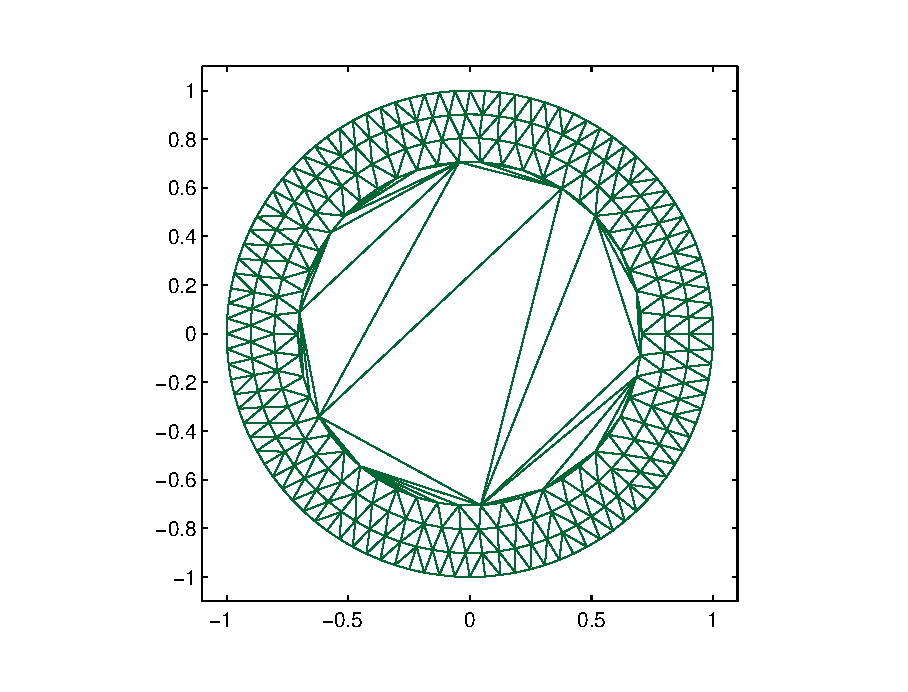
\includegraphics[width=11cm]{img/trimal.eps}
\caption{Triángulos fuera del dominio.}
\label{trimal}
\end{figure}

Para resolver este problema, simplemente eliminamos los triángulos que están fuera del dominio. ¿Cómo determinamos si un triángulo está fuera del dominio? Calculamos el centroide del triángulo. Dado un triángulo $t_1=(a_i,a_j,a_k)$, calculamos el punto $\frac{a_i+a_j+a_k}{3}$ y vemos si queda fuera del dominio, en cuyo caso eliminamos el triángulo. 
\begin{figure}[H]
\centering
\includegraphics[width=11cm]{img/tribien.eps}
\caption{Corrección de la triangulación.}
\label{tribien}
\end{figure}
Para llevar a cabo los cálculos subsecuentes requerimos tener información acerca de los triángulos y los nodos. Para cada nodo, nos interesa saber quienes son sus ``vecinos''. Dos nodos distintos $a_i,a_j$ son vecinos si $a_i$ y $a_j$ son nodos pertenecientes a un mismo triángulo.  Por ejemplo:

\begin{figure}[H]
\begin{center}
\begin{tikzpicture}[line cap=round,line join=round,>=triangle 45,x=1.0cm,y=1.0cm]
\clip(-3.35,1.04) rectangle (5.3,4.59);
\fill[color=zzttqq,fill=zzttqq,fill opacity=0.1] (-0.94,4.3) -- (-3.14,1.55) -- (4.74,3.36) -- cycle;
\draw [color=zzttqq] (-0.94,4.3)-- (-3.14,1.55);
\draw [color=zzttqq] (-3.14,1.55)-- (4.74,3.36);
\draw [color=zzttqq] (4.74,3.36)-- (-0.94,4.3);
\draw (-1.13,4.75) node[anchor=north west] {$ a_i $};
\draw (4.81,3.52) node[anchor=north west] {$a_j$};
\draw (-3.4,1.5) node[anchor=north west] {$ a_k $};
\begin{scriptsize}
\fill [color=qqqqff] (-0.94,4.3) circle (1.5pt);
\fill [color=qqqqff] (-3.14,1.55) circle (1.5pt);
\fill [color=qqqqff] (4.74,3.36) circle (1.5pt);
\end{scriptsize}
\end{tikzpicture}
\end{center}
\caption{Triángulo $t_1$.}
\label{f3_1}
\end{figure}
Si tenemos el triángulo $t_1=(a_i , a_j , a_k) $ los vecinos de $a_i$ en el triángulo $t_1$ serían $a_j$ y $a_k$. Algo que podría pasar es que en otro triángulo vuelvan a ser vecinos una pareja de nodos $t_2=(a_i , a_k , a_l)$. En este caso $a_i$ y $a_k$ vuelven a ser vecinos, pero no es el mismo triángulo. Es importante en la implementación computacional del MEF guardar para cada nodo la información de sus nodos vecinos y de los triángulos a los que pertenecen.
\begin{figure}[H]
\centering
\begin{tikzpicture}[line cap=round,line join=round,>=triangle 45,x=1.0cm,y=1.0cm]
\clip(-5.78,0.76) rectangle (5.45,5.32);
\fill[color=zzttqq,fill=zzttqq,fill opacity=0.1] (-0.94,4.3) -- (-3.14,1.55) -- (4.74,3.36) -- cycle;
\fill[color=zzttqq,fill=zzttqq,fill opacity=0.1] (-3.14,1.55) -- (-0.94,4.3) -- (-5.32,4.8) -- cycle;
\draw [color=zzttqq] (-0.94,4.3)-- (-3.14,1.55);
\draw [color=zzttqq] (-3.14,1.55)-- (4.74,3.36);
\draw [color=zzttqq] (4.74,3.36)-- (-0.94,4.3);
\draw (-1.12,4.9) node[anchor=north west] {$ a_i $};
\draw (4.74,3.85) node[anchor=north west] {$a_j$};
\draw (-3.51,1.5) node[anchor=north west] {$ a_k $};
\draw [color=zzttqq] (-3.14,1.55)-- (-0.94,4.3);
\draw [color=zzttqq] (-0.94,4.3)-- (-5.32,4.8);
\draw [color=zzttqq] (-5.32,4.8)-- (-3.14,1.55);
\draw (-5.53,5.4) node[anchor=north west] {$a_l$};
\begin{scriptsize}
\fill [color=qqqqff] (-0.94,4.3) circle (1.5pt);
\fill [color=qqqqff] (-3.14,1.55) circle (1.5pt);
\fill [color=qqqqff] (4.74,3.36) circle (1.5pt);
\fill [color=qqqqff] (-5.32,4.8) circle (1.5pt);
\end{scriptsize}
\end{tikzpicture}
\caption{Triángulos $t_1$ y $t_2$.}
\label{f3_2}
\end{figure}

Una manera de obtener dicha información es recorrer todos los nodos y encontrar a qué triángulos pertenece cada uno. Esto resulta ser muy ineficiente ya que se visitan todos los triángulos tres veces, una por cada nodo. Una manera más eficiente de encontrar los triángulos a los que pertenece un nodo dado consiste en recorrer la matriz de triángulos que nos dá el algoritmo de Delaunay y de guardar la información para cada nodo en una otra matriz; se guarda el nodo vecino y el triángulo al que pertenece en común. La matriz que se guarda es similar a la que se presenta a continuación: 

\begin{equation*}
	\begin{array}{ccccccc}
		 \text{ Nodo } & \text{ Vecino 1 } & \text{Tri\'angulo 1}& \text{ Vecino 2 } & \text{Tri\'angulo 2} & ... \\
			a_1 & a_j & t_1 & a_k & t_2 & ...\\		
			a_2 & a_l & t_3 & a_m & t_4 & ...\\
			\vdots & \vdots &\vdots &\vdots &\vdots &\ddots \\

	\end{array}
\end{equation*}

\section{Construcción del sistema de ecuaciones}

Hasta ahora sólo hemos mostrado las equivalencias entre los problemas variacionales y las ecuaciones diferenciales; no hemos expuesto como se resolverán, ni el problema que le plantearemos a la máquina para que resuelva. En esta parte hablaremos precisamente de ese paso, y además de una dificultad relacionada con el número de condición de una matriz. 
Recordemos el problema variacional que queremos resolver:

Encontrar $u\in H_0^1(\Omega)$, de tal manera que:
\[a(u,v)=\iint_\Omega \nabla u\cdot \nabla v \dxy = \iint_\Omega f v\dxy, \forall v \in H_0^1. \]
Sean $\left\lbrace x_i\right\rbrace_{i=1}^n$ nodos interiores en $\Omega$, y $\left\lbrace \phi_i\right\rbrace_{i=1}^n$, funciones nodales como las descritas en \ref{Sfn}. Sea $V_h$ el espacio generado por $\left\lbrace \phi_i\right\rbrace_{i=1}^n$. El problema que vamos a resolver numéricamente es el siguiente: 

Encontrar $\hat{u}\in V_h \subset H_0^1(\Omega)$, de tal manera que:
\[\iint_\Omega \nabla \hat{u}\cdot \nabla v \dxy = \iint_\Omega f v\dxy, \forall v \in V_h \]
Por lo cual basta encontrar los coeficientes $\llaves{\alpha_i}_{i=1}^n$ de tal manera que:
\[\iint_\Omega \nabla\left( \sum_{i=1}^n \alpha_i \phi_i\right) \cdot \nabla \phi_j \dxy = \iint_\Omega f \phi_j\dxy, \text{ para } j=1...n \]
\[\Rightarrow \sum_{i=1}^n\alpha_i \intomega{\nabla \phi_i\cdot\nabla \phi_j}=\intomega{f \phi_j}, \text{ para } j=1...n\]
\[\Rightarrow \sum_{i=1}^n\alpha_i a(\phi_i,\phi_j)=\intomega{f \phi_j}, \text{ para } j=1...n\]
Podemos escribir la igualdad anterior como un sistema lineal de ecuaciones algebraicas: 
\begin{equation}
A\xi=b,\label{algebraica}
\end{equation}
donde: \[A_{i,j}=a(\phi_i,\phi_j), \xi_i=\alpha_i\text{ y } b_i=\intomega{f\phi_i}.\]
Para calcular las entradas de la matriz $A$ del sistema se tiene lo siguiente:
\[ a(\phi_i,\phi_j)=\iint_\Omega \nabla\phi_i\cdot \nabla \phi_j \dxy =\sum_{t\in T_i\bigcap T_j} \iint_{t} \nabla\phi_i\cdot \nabla \phi_j\dxy,\]
donde $T_i$ es el conjunto de triángulos a los que el nodo $x_i$ pertenece, por lo tanto la matriz A es rala. Más adelante se proporciona una manera de calcular la matriz $A$ del sistema.

 

\section{Manejo de datos}

Como ya mencionamos, se requiere resolver un sistema de ecuaciones:
\begin{equation}\label{sisteq}
  A\xi=b.
\end{equation}
La matriz $A$ puede ser muy grande y tomar mucho espacio guardarla. Por ejemplo, para un cuadrado con 10x10 nodos necesitamos guardar una matriz de 100 x 100. Para un cuadrado con 100 x 100 nodos, se necesita una matriz de $10^4$ x $10^4$ lo cual requeriría un total de $10^8$ entradas. Afortunadamente la matriz $A$ es rala, por lo que no es necesario almacenar cada entrada.

Al analizar la estructura de la matriz $A$ notamos en primer lugar que la matriz $A_{i,j}=a(\phi_i,\phi_j)$ es simétrica:

\[ a(\phi_i,\phi_j)=\iint_\Omega \nabla \phi_i \cdot \nabla \phi_j \dxy = \iint_\Omega \nabla \phi_j \cdot \nabla \phi_i \dxy=a(\phi_j,\phi_i). \]

En segundo lugar, por el soporte compacto de las funciones nodales, podemos ver que gran parte de las entradas de la matriz $A$ son ceros. Para los dominios y triangulaciones probadas, hubo a lo más 15 vecinos en algún nodo. Por lo que en lugar de guardar toda la matriz, usamos una estructura de matriz rala; es decir, en lugar de guardarla completa, sólo guardamos las entradas distintas de cero, junto con indicadores del lugar que ocupan. Por ejemplo, si tenemos la siguiente matriz: 
\begin{equation*}
\begin{pmatrix}
		0 & 0 & 1 \\
		3 & 0 & 0 \\
		0 & 5 & 0 \\
\end{pmatrix}
\end{equation*}

Entonces sólo guardaríamos la información siguiente: 
\begin{equation*}
	\begin{array}{cccc}
		a_{i,j} & i & j\\
		1 & 1 & 3 \\
		3 & 2 & 1 \\
		5 & 3 & 2 \\
	\end{array}.
\end{equation*}

En casos más grandes, y con más ceros dentro de la matriz (como es el caso de la matriz que estamos resolviendo) el ahorro de memoria ocupada para almacenar la matriz es considerable.

Con la estructura rala se pueden programar la mayoría de los métodos iterativos para aproximar la solución del sistema (\ref{sisteq}) en esta tesis usaremos el método del Gradiente Conjugado el cual describiremos más adelante.

\section{Número de condición de la matriz $A$.}

Es de nuestro interés conocer el número de condición $\kappa(A)$ de la matriz $A$, ya que de ello dependerá en gran medida la eficiencia del algoritmo. Si la matriz $A$ del sistema (\ref{sisteq}) tiene un número de condición grande, al resolver numéricamente el sistema se puede producir pérdida de precisión. Además, un número de condición grande (y dependiendo de la distribución del los valores propios de $A$) puede producir que el método del gradiente conjugado requiera más iteraciones al aproximar la solución de (\ref{sisteq}) con una tolerancia dada al error de aproximación.

El número de condición dependerá de los triángulos que tomemos en el dominio. A continuación algunas definiciones que nos ayudarán a estimar el tamaño del número de condición de la matriz. 

Supongamos que tenemos una triangulación $T=\left \lbrace t_i\right\rbrace$. Para cada triángulo $t$, llamaremos $\rho_t$ al diámetro del círculo inscrito en $t$, por otro lado, llamaremos $h_t$, al lado más largo del triángulo $t$. Además sea $h=\max_{t\in T} \left\lbrace	h_t\right\rbrace$. (Ver Figura \ref{rhoh})

\begin{figure}[H]\label{rhoh}
\centering
\begin{tikzpicture}[line cap=round,line join=round,>=triangle 45,x=2.0cm,y=2.0cm]
\clip(1.19,3.93) rectangle (7.95,5.92);
\fill[color=qqtttt,fill=qqtttt,fill opacity=0.1] (1.28,5.57) -- (7.88,5.61) -- (4.59,4.23) -- cycle;
\draw [color=qqtttt] (1.28,5.57)-- (7.88,5.61);
\draw [color=qqtttt] (7.88,5.61)-- (4.59,4.23);
\draw [color=qqtttt] (4.59,4.23)-- (1.28,5.57);
\draw [color=qqwwtt] (4.59,4.93) circle (1.31cm);
\draw [color=qqtttt] (4.59,4.28)-- (4.58,5.59);
\draw (4.62,5.05) node[anchor=north west] {$\rho_t$};
\draw (4.55,5.9) node[anchor=north west] {$h_t$};
\end{tikzpicture}
\caption{$\rho_t$ y $h_t$.}
\end{figure}

Con estos parámetros, podemos hablar de familias de triangulaciones, $\left\lbrace T_h\right \rbrace$ es el conjunto de triangulaciones de tal manera que el lado más grande sea $h$. Suponemos que las triangulaciones $T_h$ cumplen con lo siguiente: existen constantes positivas $\beta_1,\beta_2$, independientes de $h$, de tal manera que para todo triángulo $t\in T_h$, se cumpla que: 
\begin{eqnarray}
h_t\geq \beta_1h,\\
\frac{\rho_t}{h_t}\geq \beta_2,
\end{eqnarray}
si cumple con las ecuaciones, se dice que la triangulación $T_h$, es cuasi-uniforme. Demostraremos que $\kappa(A)=O(h^{-2})$ para triangulaciones cuasi-uniformes. Para ello enunciaremos un lema:
\begin{lema}\label{lemadesig}\footnote{Para una prueba del lema, \ref{lemadesig} ver el Apéndice \ref{AN2}.}
Existen constantes $c$ y $C$, que solo dependen de $\beta_i$, tales que
\begin{eqnarray}
ch^2|\alpha |^2\leq ||v||^2\leq Ch^2 |\alpha |^2.\label{desig1}\\
\intomega{|\nabla v|^2}\leq Ch^{-2}||v||^2, \label{desig2}
\end{eqnarray}
$$\forall v\in V_h, \alpha \in \re ^n, v = \sum_{i=1}^{n}\alpha_i \phi_i $$
Donde $||v||=||v||_{\LD(\Omega)}$ y $|\alpha| $ es la norma 2 de $\re^n$.
\end{lema}
Para estimar el número de condición de la matriz con el lema \ref{lemadesig}, notemos que la matriz $A$ es simétrica y positiva definida, por ello tenemos que \[\kappa(A)=\frac{\lambda_{\max}(A)}{\lambda_{\min}(A)}=\frac{\text{Valor propio m\'as grande de } A}{\text{Valor propio m\'as chico de } A },\]
gracias a ello, lo que se debe acotar son los valores propios de la matriz. 

Notemos que si \[v=\sum_{i=1}^{n}\alpha_i \phi_i,\] entonces $a(v,v)=\alpha\cdot A \alpha,$ donde \[A_{i,j}=a(\phi_i, \phi_j).\]
Ahora por \ref{desig1} y \ref{desig2}, se obtiene:
\begin{equation}\label{desigarriba}
\frac{\alpha\cdot A \alpha}{|\alpha|^{2}}=\frac{a(v,v)}{|\alpha|^{2}}\leq Ch^{-2}\frac{||v||^2}{|\alpha|^{2}}\leq C^2 \phantom{\pi} \forall \alpha \in \re^n.
\end{equation}
Dado que:\[\intomega{v^2+|\nabla v|^2}=||v||_{\hu}\geq||v||= \intomega{v^2},\]
y por el teorema \ref{teodesig}, tenemos:
\begin{equation}\label{desigabajo}
\frac{\alpha\cdot A \alpha}{|\alpha|^{2}}=\frac{a(v,v)}{|\alpha|^{2}}\geq\frac{||v||_{\hu}}{|\alpha|^{2}}\geq\gamma\frac{||v||}{|\alpha|^{2}}\geq C\gamma h^2 \phantom{\pi} \forall \alpha \in \re^n\setminus \llaves{0}.
\end{equation}
Juntando los resultados \ref{desigarriba} y \ref{desigabajo}, resulta: 
\[ C\gamma h^2\leq\frac{\alpha\cdot A \alpha}{|\alpha|^{2}}\leq C^2. \]
Gracias a esto sabemos que los valores propios están acotados: \[\lambda_{\min}(A)\geq C\gamma h^2,\]\[\lambda_{\max}(A)\leq C^2.\]
Esto debidio a que:

\[\lambda_{\max}(A)= \max_{\alpha\in \re^n\setminus \llaves{0}}\frac{\alpha\cdot A\alpha}{ |\alpha|^2}, \]
\[\lambda_{\min}(A)= \min_{\alpha\in \re^n\setminus \llaves{0}}\frac{\alpha\cdot A\alpha}{ |\alpha|^2}. \]
Por lo tanto \[\kappa(A)\leq C' h^{-2}.\]



\section{Cuadraturas y cálculo de integrales.}

Para obtener el lado derecho de la ecuación (\ref{algebraica}) debemos calcular las siguientes integrales:

\begin{equation}
\iint_\Omega f \phi_i \dxy \text{ para } i=1...n. \label{3.1}
\end{equation}

Con la elección de funciones nodales se tiene la ventaja de que el integrando vale cero en gran parte del dominio. La región donde no es cero está partido en triángulos; hay una forma sencilla de escribir la función $\phi_i$ en cada triángulo. Por otro lado  necesitamos una manera de calcular (\ref{3.1}) numéricamente. 

Tomando en cuenta la notación de (\ref{Sfn}), debemos notar que (\ref{3.1}) se puede escribir a su vez como:
\begin{equation}
\sum_{t\in T_i }\iint_t f \phi_i \dxy \text{ para } i=1...n. \label{3.2}
\end{equation}

Por lo tanto, el cálculo de (\ref{3.1}) se reduce a calcular integrales en varios triángulos. El valor de la integral doble en cada triángulo $t$ será aproximado por una cuadratura que requiere 7 evaluaciones del integrando. A continuación describiremos esta cuadratura (ver \cite{Claes}).

Tomemos un triángulo $t=(a_1,a_2,a_3)$, llamaremos $b_1=\frac{1}{2}(a_1+a_2),b_2=\frac{1}{2}(a_2+a_3),b_3=\frac{1}{2}(a_1+a_3)$ los puntos medios entre los vértices del triángulo, y a su vez calculamos el centroide del triángulo: $ a'=\frac{1}{3}(a_1+a_2+a_3)$, y $a_t$ será el área del triángulo. Ahora sea $g$ una función cualquiera integrable. La fórmula de la cuadratura que usaremos está dada por: 

\begin{equation} 
\int_t g \dxy \sim a_t\left [ \sum_{i=1}^3\left( \frac{g(a_i)}{20} + \frac{ 2 g(b_i)}{15}\right) + \frac{9 g(a')}{20}\right ],
\label{quadrature}
\end{equation}

La fórmula de cuadratura (\ref{quadrature}) es exacta para polinomios de grado a lo más 3 (Ver \cite{Claes}). 

Hay otros métodos de integración, por ejemplo la regla de Simpson para integrar, el problema con este método en particular dentro del contexto de los elementos finitos es que se requiere calcular la integral sobre un triángulo, y la regla de simpson es muy buena cuando se tienen dominios rectangulares, por lo que en este caso particular nos conviene más usar las cuadraturas.



\section{Resolución del sistema de ecuaciones: gradiente conjugado}

Para resolver el sistema de ecuaciones requerido, usaremos el método del gradiente conjugado. El método del gradiente conjugado, resuelve de manera general y numérica un sistema de ecuaciones lineales:
\begin{equation}Ax=b,\label{axb1} \end{equation}
donde la matriz $A$ tiene que ser simétrica y positiva definida de tamaño $n$; $x,b$ vectores en $\re^n$. (Ver anexo \ref{AN1}.)
\section{Error de aproximación}

Se puede probar que el error de aproximación a la función $u$ tiene una cota, que de hecho es la siguiente( Ver \cite{Claes}): 

\[||u-u_h||_{\LD(\Omega)}\leq Ch^2||u||_{H^2(\Omega)},\]
para triangulaciones cuasi uniformes $T_h$ y $u_h$ la solución aproximada del MEF usando funciones nodales continuas y lineales por trozos.

Este error dice que entre más fina sea la partición que tomemos de $\Omega$, mejor aproximación tendremos a $u$. Como ya demostramos arriba, el problema con hacer las particiones tan pequeñas es que el número de condición de la matriz usada crece, y se complica resolver el sistema lineal que necesitamos para obtener la solución. En respuesta a esto existen métodos de precondicionamiento\footnote{Para mayor profundidad sobre el tema de precondicionamiento de la matriz, ver \cite{Claes} y \cite{Nocedal}} de la matriz $A$. El precondicionamiento es un método para encontrar o aproximar la solución $x$ de (\ref{axb1}) resolviendo un sistema con una matriz cuyo número de condición sea menor que el de $A$. 

Otra manera de resolver el sistema de ecuaciones es por medio de la factorización Cholesky, que a diferencia del método del gradiente conjugado, no es sensible al número de condición de la matriz, aunque por otro lado, puede ser un poco más lento. Ambos son usados para la resolución del sistema de ecuaciones en el MEF.

\chapter{Dimensión 1}
En este capítulo  implementaremos el MEF para problemas en dimensión 1, incluyendo una ecuación no lineal. Un ejemplo sencillo de implementación del métodoes el siguiente. Supongamos que tenemos la siguiente ecuación:
\begin{align}
-u''(x)=f(x),&\hspace{10pt} \forall x\in(0,1)\\ \label{ecdim1}
u(0)=u(1)=0.&
 \end{align}
Al tomar  el intervalo $[0,1]$ para simplificar los cálculos pero es sencillo extender el resultado a un intervalo general, de la forma $[a,b]$.

Tomemos una partición del intervalo $[0,1]$ por simplicidad será una partición uniforme:
\[0=x_0<x_1<...<x_{n+1}=1,\]
tenemos que 
\[\forall i\in \llaves{1,..., n}, x_i-x_{i-1}=h,\]
con $h$ constante.

Sea $V$ el espacio de funciones continuas y lineales a pedazos en el intervalo $[0,1]$ y $V_h$ el conjunto de funciones $v$ que cumplen con lo siguiente:
 \begin{itemize}
\item Son continuas
\item En cada intervalo $\llaves{I_i}_{i=1}^n$ son lineales.
\item $v(0)=v(1)=0$.
\end{itemize}

Las funciones nodales $\phi_i$, en este caso son funciones que pertenecen a $V_h$ y que además cumplen con: 
\[\phi_i(x_j)=\left\lbrace\begin{array}{cc} 1 & \text{ si } i=j\\ 0&\text{ si }i\neq j\end{array}\right. .\]
Para poder ilustrar mejor el concepto de las funciones nodales en dimensión 1, ver la gráfica de la figura \ref{philineal}.
\begin{figure}[H]
\centering
\begin{tikzpicture}[line cap=round,line join=round,>=triangle 45,x=8.0cm,y=8.0cm]
\draw[->,color=black] (-0.07,0) -- (1.6,0);
\foreach \x in {,0.2,0.4,0.6,0.8,1,1.2,1.4,1.6}
\draw[->,color=black] (0,-0.1) -- (0,0.59);
\foreach \y in {,0.2,0.4}
\clip(-0.07,-0.1) rectangle (1.6,0.59);
\draw [color=qqwwtt] (0.5,0)-- (1,0.5);
\draw [color=qqwwtt] (1,0.5)-- (1.5,0);
\draw (0.47,0) node[anchor=north west] {$x_{i-1} $};
\draw (1.47,0) node[anchor=north west] {$ x_{i+1}$};
\draw (0.99,0.0) node[anchor=north west] {$ x_i $};
\draw (-0.08,0.54) node[anchor=north west] {1};
\draw (0.75,0.0) node[anchor=north west] {$h$};
\draw (1.26,0.0) node[anchor=north west] {$h$};
\draw [line width=1.2pt,dotted,color=qqwwtt] (1,0.5)-- (0,0.49);
\draw [color=qqwwtt] (1.01,0)-- (1.01,0.03);
\begin{scriptsize}
\fill [color=qqwwtt] (0.5,0) circle (1.5pt);
\fill [color=qqwwtt] (1,0.5) circle (1.5pt);
\fill [color=qqwwtt] (1.5,0) circle (1.5pt);
\fill [color=qqwwtt] (1,0.5) circle (1.5pt);
\fill [color=qqwwtt] (0,0.49) circle (1.5pt);
\end{scriptsize}
\end{tikzpicture}
\caption{$\phi_i$.}
\label{philineal}
\end{figure}
Para resolver la ecuación transformamos el problema (\ref{ecdim1}) en uno variacional discretizado. El problema en forma variacional es encontrar $\hat{u} \in V_h$, de tal forma que:
\[\icu\hat{u}'(x)v'(x)\dx=\icu f(x)v(x)\dx, \forall v \in V_h,\]
que es equivalente a encontrar los coeficientes $\xi_i$ de tal manera que:
\[\icu\sum_{i=1}^n\xi_i \phi_i'(x)\phi_j'(x)\dx=\icu f(x)\phi_j(x)\dx, \text{ para } j=1...n\]
\[\Rightarrow\sum_{i=1}^n\xi_i \icu \phi_i'(x)\phi_j'(x)\dx=\icu f(x)\phi_j(x)\dx, \text{ para } j=1...n. \]
Ahora estudiemos el término $\displaystyle\icu \phi_i'(x)\phi_j'(x)\dx $. Podemos ver en la figura \ref{philineal} que las funciones $\phi_i$ se anulan en gran parte del dominio, por lo mismo, la integral es sencilla de calcular: 

$$\icu \phi_i'(x)\phi_j'(x)\dx =0 \text{ si } |i-j|>1,$$
por otro lado tenemos tres casos distintos, $j=i-1,1,i+1$:
\begin{itemize}
\item $j=i-1$
$$\icu\phi_{i-1}'(x)\phi_{i}'(x)\dx=\int_{x_{i-1}}^{x_{i}}\phi_{i-1}'(x)\phi_{i}'(x)\dx$$
$$=\int_{x_{i-1}}^{x_{i}}-\frac{1}{h}\frac{1}{h}= -\frac{(x_i-x_{i-1})}{h^2}\dx= -\frac{1}{h}.$$
\item $j=i$
$$\icu\phi_{i}'(x)\phi_{i}'(x)\dx=\int_{x_{i-1}}^{x_{i+1}}\phi_{i}'^2(x)\dx$$
$$=\int_{x_{i-1}}^{x_{i}}\phi_j'^2(x)\dx+\int_{x_{i}}^{x_{i+1}}\phi_j'^2(x)\dx $$
$$= \int_{x_{i-1}}^{x_{i}}\frac{1}{h^2}\dx+\int_{x_{i}}^{x_{i+1}}\frac{1}{h^2}\dx $$
$$=\frac{(x_i-x_{i-1})}{h^2}+\frac{(x_{i+1}-x_{i})}{h^2} = \frac{2h}{h^2}=\frac{2}{h}.$$
\item $j=i+1$
$$\icu\phi_{i+1}'(x)\phi_{i}'(x)\dx=\int_{x_{i}}^{x_{i+1}}\phi_{i+1}'(x)\phi_{i}'(x)\dx$$
$$=\int_{x_{i}}^{x_{i+1}}-\frac{1}{h}\frac{1}{h}= -\frac{(x_{i+1}-x_{i})}{h^2}\dx= -\frac{1}{h}.$$
\end{itemize}

Por lo que la matriz $A$ queda como sigue:
$$A=\frac{1}{h}\left[
\begin{array}{ccccc}
2&-1&0&0&...\\
-1&2&-1&0&...\\
0&-1&2&-1&...\\
\vdots&\vdots&\vdots&\vdots&\ddots
\end{array}\right].$$
El sistema de ecuaciones a resolver:
\[A\xi=b,\]
donde $\xi_i$ es el vector de coeficientes a encontrar y \[b_i=\icu f(x)\phi_i(x)\dx\]es el lado derecho del sistema.
Ejemplificaremos el funcionamiento del algoritmo con un problema muy sencillo. Considerar el problema con valores en la frontera
\begin{eqnarray*}
-u''(x)=\pi^2\sen(\pi x)\\
u(0)=u(1)=0
\end{eqnarray*}
En este caso se puede calcular la solución exacta, \[u(x)=\sen(\pi x),\]la cual usaremos para analizar el grado de precisión de la solución aproximada. 
Tomando 11 nodos se obiene el siguiente sistema de ecuaciones:
\[10 \left[
\begin{array}{ccccc}
2&-1&0&0&...\\
-1&2&-1&0&...\\
0&-1&2&-1&...\\
\vdots&\vdots&\vdots&\vdots&\ddots
\end{array}\right] \xi=b.\]
\[b_i=\icu \sen(x)\phi_i(x)\dx\]
La solución la podemos apreciar en la figura \ref{fig:sin10nod}, y en el acercamiento de la figura \ref{fig:asin10nod} podemos apreciar el error asociado a la aproximación lineal de la función $\sen(x)$.
\begin{figure}[H]
\centering
\includegraphics[width=10cm]{img/sin10nod.png}
\caption{$u(x)$ y $\hat{u}(x)$.}
\label{fig:sin10nod}
\end{figure}
\begin{figure}[H]
\centering
\includegraphics[width=10cm]{img/acercamientosin10nod.png}
\caption{$u(x)$ y $\hat{u}(x)$.}
\label{fig:asin10nod}
\end{figure}

\section{Ecuaciones diferenciales no lineales.}
Para ilustrar un poco más la flexibilidad del MEF, desarrollaremos para el caso unidimensional una extensión del mismo para resolver ecuaciones diferenciales no lineales, en particular ecuaciones de la forma: 
\begin{eqnarray}
-u''(x)+g(u(x))=f(x) \\ \label{nleq1}
u(a)=0,\text{ } u(b)=0
\end{eqnarray}
De nuevo, para resolver (\ref{nleq1}), aproximaremos $u$, con una base de funciones como la que se ilustra en la figura \ref{philineal}, de tal manera que:
\[u(x)\approx\hat{u}(x)=\sum_{i=1}^n\alpha_i\phi_i(x).\]
Para aproximar la ecuación seguimos el mismo procedimiento que hemos seguido hasta el momento para discretizar las ecuaciones diferenciales: sea $\phi_j(x)$ una elemento de la base del espacio $V_h$. Tomamos la ecuación \ref{nleq1} y la multiplicamos por $\phi_j$ e integramos sobre el intevalo $[a,b]$ y nos queda lo siguiente: 
\[-\int_a^b \hat{u}''(x)\phi_j(x)\dx+\int_{a}^b g(\hat{u}(x)) \phi_j(x)=\int_a^bf(x)\phi_j(x)\dx\]
\begin{equation}
\Rightarrow\int_a^b \hat{u}'(x)\phi_j'(x)\dx+\int_{a}^b g(\hat{u}(x)) \phi_j(x)=\int_a^bf(x)\phi_j(x)\dx\label{nleq2}
\end{equation}
En el caso lineal, la ecuación (\ref{nleq2}) daba lugar a un sistema lineal de ecuaciones. En este caso el sistema es no lineal.

Para resolver la ecuación (\ref{nleq2}) se plantea un sistema de ecuaciones no lineales. Tendremos una ecuación por cada $\phi_j$ en la base, por lo que tendremos $n$ ecuaciones no lineales con $n$ incógnitas: $\alpha_j$. El sistema a resolver es el siguiente:
\begin{equation}
F(\boldsymbol\alpha)=\textbf{0}\label{nleq3}
\end{equation} 
Donde $F:\re^n\rightarrow\re^n$ y se puede expresar entrada a entrada como sigue: 
\[F_j(\boldsymbol\alpha)=\int_a^b\hat{u}'(x)\phi'_j(x)\dx+\int_a^b g(\hat{u}(x)) \phi_j(x)\dx-\int_a^b f(x) \phi_j(x)\dx,\]
es claro que si $F(\boldsymbol\alpha)=\boldsymbol 0$ entonces:
\[\int_a^b\hat{u}'(x)\phi'_j(x)\dx+\int_a^b g(\hat{u}(x)) \phi_j(x)\dx=\int_a^b f(x) \phi_j(x)\dx,\]
que al sustituir $\hat{u}(x)$ por $\sum_{i=1}^n\alpha_i\phi_i(x)$ queda como sigue: 
\[\int_a^b\left(\sum_{i=1}^n\alpha_i\phi_i(x)\right)'\phi'_j(x)\dx+\int_a^b g\left(\sum_{i=1}^n\alpha_i\phi_i(x)\right) \phi_j(x)\dx=\int_a^b f(x) \phi_j(x)\dx.\]


\subsection{Método de Newton} 

El algoritmo de Newton\footnote{ Ver \cite{Nocedal} } es un método iterativo, usado para aproximar una solución del sistema no lineal (\ref{nleq3}). El método parte de una aproximación inicial $x_0$ dada. Se calculan nuevas aproximaciones $x_1,x_2,...$ con la fórmula
\[J_F(x_{k})(x_{k+1}-x_k)=-F(x_k),\]
dada la aproximación $x_k$. Por lo que la aproximación $x_{k+1}$ se obtiene resolviendo un sistema lineal de ecuaciones. 

El algoritmo se detendrá cuando $F(x_k)$ sea menor a una tolerancia preestablecida, que en el caso del algoritmo programado es $10^{-9}$. 

Por otro lado para aproximar $J_F(x_k)$ se usa la siguiente fórmula:

\[(J_F(x_k))_{\cdot,i}\approx\frac{F(x_k+he_i)-F(x_k-he_i)}{2h}, \]

donde $h\in \re$ es constante y pequeña, en este caso de orden $10^{-3}$. Mientras que $e_i\in \re^n$ es el vector que tiene cero en todas las entradas excepto en la $i$-ésima donde vale 1.

En muchos casos el método de Newton nos ayuda a resolver la ecuación \ref{nleq3} a una velocidad de convergencia cuadrática. Para el caso de este trabajo el punto inicial se tomó con puntos sobre la línea que una $(a,u(a)),(b,u(b))$.

Como hemos ejemplificado, el método de elementos finitos es muy flexible y aplicable a otro tipo de ecuaciones, variando tanto el espacio al que pertenece, como el tipo de problema. 

Por ejemplo, podríamos usar en lugar de las bases lineales que hemos usado hasta ahora, bases cuadráticas, e inclusive con mayores grados de polinomio. Dependiendo del grado del polinomio en las bases dependerán las características que podremos aproximar de $u$. Por ejemplo, podríamos estimar $u'(x)$, si usásemos polinomios cúbicos. 

\chapter{Resultados numéricos}

En este capítulo presentaremos resultados numéricos de algunos ejemplos. La manera de medir el error será la siguiente: 
\[ \text{err}(\alpha)=\frac{||\alpha - u(\hat{x})||}{||u(\hat{x})||},\]
donde $\alpha$ es el vector de aproximaciones con el MEF en los nodos, $\hat{x}=(x_1,...x_n)$ es el vector de nodos $\lbrace x_1,...,x_n\rbrace$ y $u(\hat{x})=(u(x_1),u(x_2),...,u(x_n))$  . En los ejemplos presentados conocemos la solución exacta al problema, sin embargo las pruebas nos servirán para poder observar el comportamiento del método. La máquina en la que se hicieron las pruebas tiene un procesador con 4 núcleos a 200 GHz, 8gb de memoria RAM, en un sistema operativo Ubuntu, con Matlab.  

Dado el problema: Encontrar $u$ tal que: 
\begin{align}
\label{eje1}
-\Delta u &= f \hspace{10 pt} \text{en } \Omega \subset \re^2 ,\\ 
u &=g \hspace{10 pt} \text{en } \Gamma=\partial\Omega. 
\end{align}

Primer ejemplo: 
\[\Omega =[0,1]\times[0,1],\]\[g(x,y)=0.\]\[ f(x,y) = - 2 \pi ^2 \sen(\pi x)\sen(\pi y).\]
En este caso sabemos que la solución es: \[ u(x,y)=\sen(\pi x)\sen(\pi y),\]
este problema no explota realmente la fortaleza del método, el dominio es sencillo, pero es un buen inicio para ver cómo se comporta. Para resolverlo, tomamos 2,500 nodos dentro del cuadrado; en estos puntos es donde encontraremos el valor aproximado de la función $u$ ($\alpha\in \re^{2500}$). En este ejemplo el error que se obtuvo fue del orden de $4.54x10^{-4}$ con un tiempo de 5.3 segundos. En el siguiente ejemplo se ilustra un caso en el que la solución no se anula en la frontera.

\begin{figure}[H]
\centering
\includegraphics[width=10cm]{img/u1a.png}
\caption{Gráfica de la solución exacta.}
\end{figure}

Las funciones para el siguiente problema son las mismas a excepción de $g$ no es cero: 
\[\Omega =[0,1]\times[0,1],\]\[g(x,y)=2x-y.\]\[ f(x,y) = - 2 \pi ^2 \sen(\pi x)\sen(\pi y).\]
La solución al problema es: \[ u(x,y)=\sen(\pi x)\sen(\pi y)+2x-y,\]

De nuevo, tomaremos 2,500 nodos dentro del cuadrado.
\begin{figure}[H]
\centering
\includegraphics[width=8cm]{img/u2r.png}
\caption{Gráfica de la solución exacta.}
\end{figure}

En este ejemplo el error es del orden de $1.94x10^{-4}$ de nuevo con un tiempo de 5.3 segundos que no es de sorprender que tengan el mismo tiempo ya que tienen el mismo número de variables.

En el siguiente ejemplo se usará un anillo como región donde se define la ecuación diferencial, a diferencia del cuadrado en los dos primeros ejemplos. en este caso la región está dada por:
\[ \left \lbrace x \in \re^2 \middle| \frac{1}{2} \leq ||x||^2_2\leq 1\right\rbrace.\]
\begin{figure}[H]
\centering
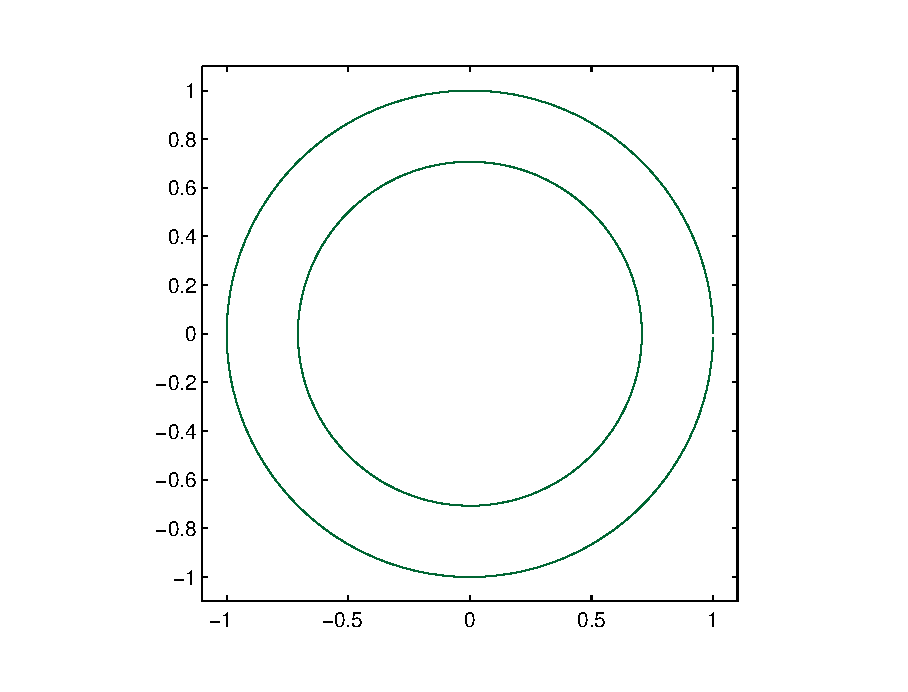
\includegraphics[width=11cm]{img/dona.eps}
\caption{Representación visual de $\Omega$.}
\end{figure}
Las funciones $f$ y $g$ de la ecuación (\ref{eje1}) son:
\begin{equation}f(x,y) = 16\pi (x^2+y^2) \sen \left(2\pi\left(x^2+y^2-\frac{1}{2}\right)\right)-8\pi \cos \left(2\pi\left(x^2+y^2-\frac{1}{2}\right)\right)\label{donaprob}\end{equation}
\[g(x,y)=2x-y.\]
De nuevo se conoce la solución al problema, para obtener el error de aproximación:
\[u(x,y)=\sen\left(2\pi\left(x^2+y^2-\frac{1}{2}\right)\right) + 2x-y. \]
Para este ejemplo, tomaremos 1,000 puntos dentro del anillo. 
El método no tiene mayor problema con el nuevo conjunto $\Omega$ y se adapta bien para conjuntos no tan sencillos. El error obtenido es del orden de $7.9x10^{-4}$ con un tiempo de procesamiento de 3.4 segundos. La figura \ref{fig:solucion}, muestra cómo se ve la solución de la ecuación; mientras que la figura \ref{fig:triang} muestra la trianguación dada para el dominio.
\begin{figure}[H]
\centering
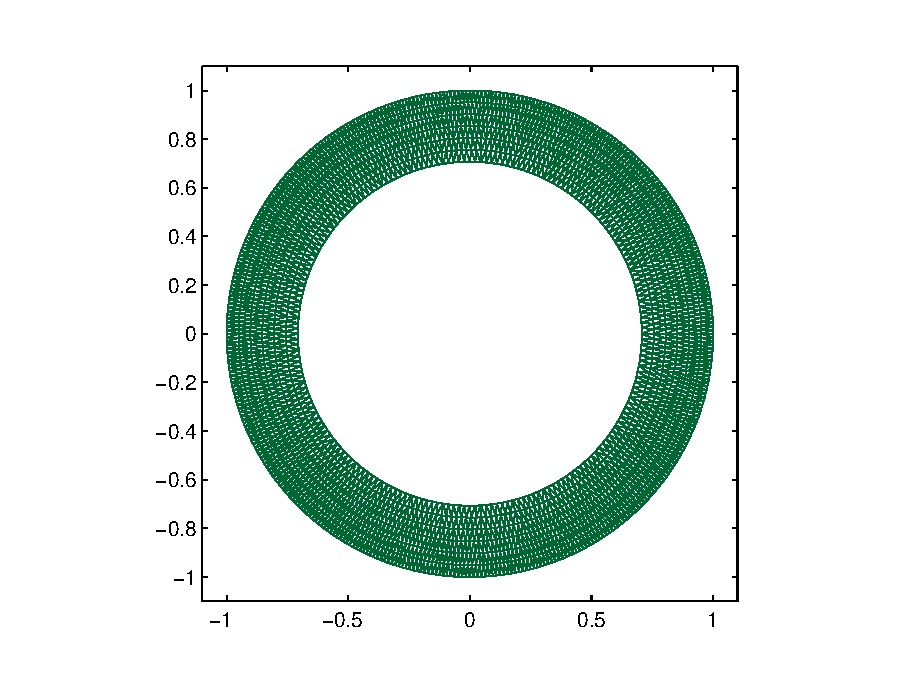
\includegraphics[width=11cm]{img/triang.eps}
\caption{Triangulación de el dominio.}
\label{fig:triang}
\end{figure}
\begin{figure}[H]
\centering
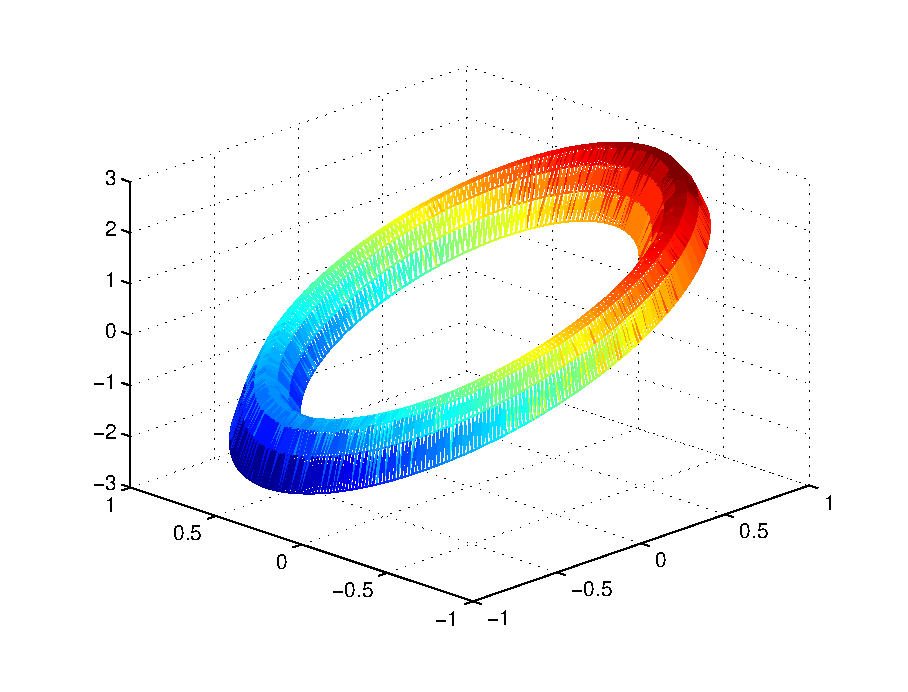
\includegraphics[width=11cm]{img/u3a.eps}
\caption{Gráfica de la solución.}
\label{fig:solucion}
\end{figure}


\chapter{Conclusiones}

\vspace{2 cm}

Un problema de aplicación requiere muchas herramientas para ser resuelto, una de ellas es la creatividad para poder conjuntar las diferentes disciplinas necesarias para resolverlo. El MEF es una gran representación de esta creatividad, ya que se logra hacer un puente entre distintas áreas de las matemáticas. Al hacer esta conjunción se puede obtener una solución tanto útil como práctica.

En principio el problema de la resolución de ecuaciones diferenciales parciales aquí tratado, es encontrar una función, un elemento que ``vive'' en un espacio de dimensión infinita. Gracias a la formulación variacional se puede hacer una discretización, que reduce el problema en otro de dimensión finita. Con la discretización se hace posible el poder manejar el problema dentro de una computadora con lo que se incrementa la capacidad de resolución a problemas mucho más grandes y complejos. 

El manejo de cualquier problema matemático en una computadora implica ciertas limitaciones, algunas pueden ser superadas estudiando y explotando las características de cada problema. En el caso presentado, se solucionó el manejo de matrices muy grandes aprovechando la estructura de las mismas: se almacenó de una manera diferente y eficiente por ser éstas ralas. Asimismo, se procuró utilizar métodos eficientes en el cálculo de integrales que, aunado a la estructuración en el dominio de las funciones utilizadas, permiten realizar un cálculo muy bueno incluso frente a dominios irregulares.

El dominio $\Omega$ de la función es una característica fundamental tanto en el problema como en la solución. El MEF triangula el dominio, haciendo más flexible la aproximación del mismo, dando así una mejor representación. El tipo de triangulación usada en esta tesis es cuasi uniforme, pero para algunos dominios más complicados se pueden usar triangulaciones localmente cuasi-uniformes.

El MEF implementado puede ser ampliado de varias maneras. Es posible cambiar la base de funciones $\lbrace\phi_i\rbrace$ a una que contenga funciones más generales, por ejemplo, aumentando el grado del polinomio usado. Esto afecta de forma directa el cálculo de las integrales y la precisión, ganando así un menor error de aproximación. En algunas aplicaciones será necesario representar dominios de mayor dimensión, de tal manera que $\Omega\subset\re^3$. El MEF implementado puede adaptarse utilizando polígonos en el espacio en lugar de triángulos. Esto significa aumentar la complejidad de cálculo y el tamaño del problema, ya que se tienen que tomar en cuenta conceptos de volumen y orientación, pero con el MEF es posible. Además, como ya se mencionó, se puede generalizar el tipo de ecuaciones resueltas a parabólicas o como se mencionó en el capítulo 4, a ecuaciones diferenciales no lineales. 

El tener un algoritmo implementando el MEF brinda la posiblidad de resolver una enorme gama de problemas en muchas disciplinas distintas. El dinamismo que posee el método es enorme. Este trabajo brinda ejemplos para una y dos dimensiones con un error de aproximación bastante bueno. La disminución del error, la mejora en el cálculo y la extensión a otras dimensiones o bases serían elementos fácilmente implementables siguiendo los detalles teóricos y técnicos aquí expuestos.

\appendix
\chapter{Algoritmo de Delaunay}\label{DelaunayApendice}
Para encontrar las triangulaciones necesarias para el desarrollo de este trabajo, como ya mencionamos, se usó el algoritmo de Delaunay. Dicho algoritmo cuenta con ciertas características que son muy deseables para el desarrollo del MEF; tiene también algunas desventajas, mismas que han sido resueltas dentro del algoritmo hecho. 

La característica principal que ayuda al desarrollo del MEF es que el algoritmo de Delaunay, maximiza el mínimo de los ángulos de todos los triángulos en la triangulación. Lo que esto garantiza es que el número de condición de la matriz $A$ que usamos en el MEF, tendrá el número de condición máximo posible para un conjunto de puntos en $\Omega$. Una desventaja del algoritmo de Delaunay es que no puede tomar en cuenta dominios como el que presentamos en esta tesis para el ejemplo (\ref{donaprob}) donde $\Omega$ no es convexo, pero esta limitante la saltamos como explicamos en la sección (\ref{Triangulacion}). 
\begin{defi}[Condición de Delaunay.]
Se dice que una triangulación cumple con la \textbf{condición de Delaunay} si ninguno de los circuncírculos de los triángulos pertenecientes a la misma, contiene otros nodos en el interior. 
\end{defi}

La triangulación final debe cumplir la \textbf{condición de Delaunay}. Un ejemplo con cuatro nodos que ilustra la condición de Delaunay:

\begin{figure}[H]
\centering
\begin{tikzpicture}[line cap=round,line join=round,>=triangle 45,x=1.5cm,y=1.5cm]
\clip(5.72,6.58) rectangle (12.36,11.43);
\fill[color=mycolor1,fill=mycolor1,fill opacity=0.1] (8.89,11.14) -- (7.63,8.44) -- (9.05,6.8) -- (10.39,8.42) -- cycle;
\fill[color=mycolor1,fill=mycolor1,fill opacity=0.1] (18.41,9.63) -- (17.15,6.93) -- (18.57,5.29) -- (19.91,6.91) -- cycle;
\draw [color=mycolor1] (8.89,11.14)-- (7.63,8.44);
\draw [color=mycolor1] (7.63,8.44)-- (9.05,6.8);
\draw [color=mycolor1] (9.05,6.8)-- (10.39,8.42);
\draw [color=mycolor1] (10.39,8.42)-- (8.89,11.14);
\draw [color=mycolor1] (8.89,11.14)-- (9.05,6.8);
\draw [color=mycolor1] (18.41,9.63)-- (17.15,6.93);
\draw [color=mycolor1] (17.15,6.93)-- (18.57,5.29);
\draw [color=mycolor1] (18.57,5.29)-- (19.91,6.91);
\draw [color=mycolor1] (19.91,6.91)-- (18.41,9.63);
\draw [color=mycolor1] (17.15,6.93)-- (19.91,6.91);
\draw [dotted,color=mycolor1] (9.94,9) circle (3.57cm);
\draw [dotted,color=mycolor1] (8.12,8.94) circle (3.5cm);
\draw [dotted,color=mycolor1] (18.53,6.69) circle (2.1cm);
\draw [dotted,color=mycolor1] (18.54,7.92) circle (2.56cm);
\begin{scriptsize}
\fill [color=mycolor1] (7.63,8.44) circle (1.5pt);
\fill [color=mycolor1] (8.89,11.14) circle (1.5pt);
\fill [color=mycolor1] (9.05,6.8) circle (1.5pt);
\fill [color=mycolor1] (10.39,8.42) circle (1.5pt);
\fill [color=mycolor1] (17.15,6.93) circle (1.5pt);
\fill [color=mycolor1] (18.41,9.63) circle (1.5pt);
\fill [color=mycolor1] (18.57,5.29) circle (1.5pt);
\fill [color=mycolor1] (19.91,6.91) circle (1.5pt);
\end{scriptsize}
\end{tikzpicture}
\caption{Triangulación de cuatro nodos que no cumple la condición de Delaunay.}
\label{fig:flip}
\end{figure}

\begin{figure}[H]
\centering
\begin{tikzpicture}[line cap=round,line join=round,>=triangle 45,x=1.5cm,y=1.5cm]
\clip(16.51,5.09) rectangle (20.4,9.7);
\fill[color=mycolor1,fill=mycolor1,fill opacity=0.1] (8.89,11.14) -- (7.63,8.44) -- (9.05,6.8) -- (10.39,8.42) -- cycle;
\fill[color=mycolor1,fill=mycolor1,fill opacity=0.1] (18.41,9.63) -- (17.15,6.93) -- (18.57,5.29) -- (19.91,6.91) -- cycle;
\draw [color=mycolor1] (8.89,11.14)-- (7.63,8.44);
\draw [color=mycolor1] (7.63,8.44)-- (9.05,6.8);
\draw [color=mycolor1] (9.05,6.8)-- (10.39,8.42);
\draw [color=mycolor1] (10.39,8.42)-- (8.89,11.14);
\draw [color=mycolor1] (8.89,11.14)-- (9.05,6.8);
\draw [color=mycolor1] (18.41,9.63)-- (17.15,6.93);
\draw [color=mycolor1] (17.15,6.93)-- (18.57,5.29);
\draw [color=mycolor1] (18.57,5.29)-- (19.91,6.91);
\draw [color=mycolor1] (19.91,6.91)-- (18.41,9.63);
\draw [color=mycolor1] (17.15,6.93)-- (19.91,6.91);
\draw [dotted,color=mycolor1] (9.94,9) circle (3.57cm);
\draw [dotted,color=mycolor1] (8.12,8.94) circle (3.5cm);
\draw [dotted,color=mycolor1] (18.53,6.69) circle (2.1cm);
\draw [dotted,color=mycolor1] (18.54,7.92) circle (2.56cm);
\begin{scriptsize}
\fill [color=mycolor1] (7.63,8.44) circle (1.5pt);
\fill [color=mycolor1] (8.89,11.14) circle (1.5pt);
\fill [color=mycolor1] (9.05,6.8) circle (1.5pt);
\fill [color=mycolor1] (10.39,8.42) circle (1.5pt);
\fill [color=mycolor1] (17.15,6.93) circle (1.5pt);
\fill [color=mycolor1] (18.41,9.63) circle (1.5pt);
\fill [color=mycolor1] (18.57,5.29) circle (1.5pt);
\fill [color=mycolor1] (19.91,6.91) circle (1.5pt);
\end{scriptsize}
\end{tikzpicture}
\caption{Triangulación de cuatro nodos que cumple la condición de Delaunay.}
\label{fig:del1}
\end{figure}

Con estas dos figuras ilustramos cómo se cumple la condición de Delaunay, pero a la vez ilustramos un concepto que se refiere a la reflexión, y con ello también un algoritmo sencillo para generar una triangulación con las características deseadas. Por supuesto hay algoritmos más complicados y eficientes, pero esto queda fuera del alcance de este documento. 

La manera más directa para generar una triangulación es agregar un vértice a la vez y retriangular las partes cercanas a este nodo, luego para cada triángulo que no cumpla con la condición de delaunay reflejarlo. Así sucesivamente hasta tener la triangulación completa. Para ahondar más en los algoritmos y en la teoría relacionada con la triangulación Delaunay, ver \cite{geobook} y \cite{delaunay}.

\chapter{Método del gradiente conjugado.}\label{AN1}

El método del gradiente conjugado, resuelve un sistema de ecuaciones lineales:
\begin{equation}Ax=b,\label{axb},\end{equation}
con $A$ simétrica y positiva definida, dando una serie de ``pasos'', acercándose en cada uno a la solución. Para resolver el sistema (\ref{axb}) se plantea el siguiente problema de minimización: 
\[\phi(x)=\frac{1}{2} x^T Ax - b^Tx.\]
Como la matriz $A$ es simétrica y positiva definida, sabemos que $x^T Ax>0\phantom{\pi} \forall x \in \re^n $. El siguiente problema es equivalente a nuestro problema original \ref{axb}:
Encontrar $x\in \re^n$ tal que:
\begin{equation} \phi(x)= \min_{z\in\re^n} \phi (z) \label{mingradconj}
\end{equation}
Sabemos que al derivar nos queda lo siguiente: 
\[\nabla\phi(x)= Ax-b=r(x)\]
sabemos por condición de suficiencia que si $\nabla\phi(x')=0 $ entonces $x'$ es un mínimo local, despejando, tenemos que $Ax'=b$ y por el hecho de que $A$ es positiva definida se puede probar que el mínimo de $\phi$ se detienen en $x=x'$. Resumiendo, para resolver el sistema de ecuaciones $Ax=b$ podemos resolver equivalentemente el problema \ref{mingradconj}. 

El método del gradiente conjugado, genera una base \textit{conjugada} de $\re^n$ con respecto a la matriz simétrica positiva definida $A$. Por vectores conjugados con respecto a una matriz $A$ entenderemos lo siguiente. \begin{defi}Sean $\lbrace p_1,...,p_n\rbrace$ vectores en $\re^n$ distintos de cero, decimos que este conjunto de vectores son conjugados con respecto a la matriz simétrica positiva definida $A$ si:
\begin{eqnarray} 
p_i^TAp_j=0 & \text{para todo } i\neq j.
\end{eqnarray}
\end{defi}

Consecuencia de esta propiedad es la ortogonalidad de los vectores: \begin{teo} \label{teogc} Si el conjunto $\lbrace p_1,...,p_n\rbrace$ es conjugado con respecto a la matriz $A$, simétrica y positiva definida, entonces el conjunto es linealmente independiente. \end{teo} 
\begin{proof} Tomemos una combinación lineal de los vectores y la igualamos a cero: 
\begin{eqnarray*} 
		&\sum_{i=1}^n\alpha_ip_i &=0 \\
\Rightarrow &\sum_{i=1}^n\alpha_ip_i\cdot A &=0 \cdot A=0\\ 
\Rightarrow &\sum_{i=1}^n\alpha_ip_i^T\cdot A^T &=0 \\
\Rightarrow & \left(\sum_{i=1}^n\alpha_ip_i^T\cdot A^T\right)\cdot \sum_{i=1}^n\alpha_ip_i &=0 \\
\Rightarrow &\sum_{i=1}^n\left(\alpha_i^2\right)\left(p_i^T\cdot A^T\cdot p_i\right)+\sum_{i\neq j}\left(\alpha_i\alpha_j\right)\cdot \left(p_i\cdot A\cdot p_j \right)&=0 \\
\end{eqnarray*}
Ahora, sabemos que como $A$ es simétrica y positiva definida, tenemos que $p_i^T\cdot A^T\cdot p_i>0$. Además por que es un conjunto conjugado con respecto a la matriz $A$, tenemos también que $p_i\cdot A\cdot p_j=0$ si $i\neq j$. Por lo tanto tenemos lo siguiente: 
\[ \sum_{i=1}^n\left(\alpha_i^2\right)=0\Rightarrow \alpha_i=0 \phantom{\pi} \forall i=1...n\]
Por lo tanto, los vectores son linealmente independientes.
\end{proof}
Presento a continuación el algoritmo del gradiente conjugado programado para esta tesis:

\begin{algorithm}[H]
\caption{Método del gradiente conjugado.}
\label{121}
\begin{algorithmic}[1]
    \State Dado $x_0$ punto inicial para el método.
    \State $r_0\leftarrow Ax_0-b$.
    \State $p_0\leftarrow -r_0$.
    \State $k\leftarrow 0$.
    \While {$r_k>10^{-10}$}
        \State $\alpha_k \leftarrow \frac{r_k'r_k}{p_k'Ap_k}$.
        \State $x_{k+1} \leftarrow x_k + \alpha_kp_k$.
        \State $r_{k+1}\leftarrow r_k+\alpha_kAp_k$.
        \State $\beta_{k+1}\leftarrow \frac{r_{k+1}'r_{k+1}}{r_{k}'r_{k}}$.
        \State $p_{k+1} \leftarrow -r_{k+1}+\beta_{k+1}p_k$
        \State $k\leftarrow k+1$.
	\EndWhile
	\State Return $x_{k+1}$
\end{algorithmic}
\end{algorithm}
El algoritmo \ref{121} converge a la solución de nuestro sistema de ecuaciones en un número acotado de pasos; el siguiente teorema del libro \cite{Nocedal} nos dice que son a los más $n$: \begin{teo}Para cualquier $x_0\in\re^n$, la secuencia generada por el algoritmo \ref{121} converge a la solución $x^*$ del sistema \ref{axb} lineal en a lo más $n$ pasos. \end{teo}

\chapter{Prueba del lema 3.1 }\label{AN2}

Para demostrar \ref{lemadesig}, probaremos que para cada triángulo $t\in T$, con vértices $a_i$ y $v\in P_1(t)$, se cumple lo siguiente:
\begin{eqnarray}
ch_t^2\sum_{i=1}^3|v(a_i)|^2\leq ||v||_{\LD(t)}\leq Ch_t^2\sum_{i=1}^3|v(a_i)|^2\label{desigabajo1}\\
\iint_t|\nabla v|^2 \dxt\leq Ch^{-2} \iint_t |v|^2\dxt\label{desigarriba1}
\end{eqnarray}
El lema resulta al sumar sobre todos los triángulos $t\in T$, que resulta claro para la desigualdad \ref{desigarriba1}, pero no necesariamente tan claro para \ref{desigabajo1}:
\[ch^2|\alpha|^2=\beta_1h^2\sum_{i=1}^n\alpha_i^2\leq \beta_1h^2c\sum_{i=1}^nn_i\alpha_i^2\leq \sum_{t\in t}ch_t^2\sum_{i=1}^3|v(a_i)|^2 \alpha_i^2,\]donde $n_i\geq1$ es el número de triángulos a los que pertenece el nodo $i$, mientras que también podemos acotar: 
\[\sum_{t\in t}Ch_t^2\sum_{i=1}^3|v(a_i)|^2\leq Ch^2\sum_{i=1}^n n_i\alpha_i^2\leq Ch^2n\sum_{i=1}^n\alpha_i^2=Ch^2n|\alpha|^2.\]
Por lo que bastará probar \ref{desigabajo1} y \ref{desigarriba1}, para ello demostraremos que se cumplen en un triángulo de ``referencia'', luego generalizando el resultado, para cualquier triángulo dado.

Sea $t'=\llaves{(0,0),(0,1),(1,0)}$ nuestro triángulo de referencia, y $\llaves{\lambda_i}_{i=1}^3$ base de $P_1(t')$. Tenemos además que para cada $\lambda_i$, podemos encontrar un índice $j$ de tal manera que $\phi_j\big|_{t'}=\lambda_i$. Tenemos que cualquier función lineal dentro del triángulo, puede ser descrita como combinación lineal de la base presentada: $$\hat{v}=\sum_{i=1}^3\hat{\alpha}_i\hat{\lambda}_i (\hat{x}_i), \phantom{\pi}\hat{x}\in t'.$$ 

Para encontrar las cotas deseadas, debemos definir algunas funciones auxiliares:
\begin{align}
 f_1(\hat{\alpha})&=\iint_t|\nabla\hat{v}|^2 \dxhat, \\
 f_2(\hat{\alpha})&=\iint_t\hat{v}^2 \dxhat, \\
 f_3(\hat{\alpha})&=\sum_{i=1}^3\hat{\alpha}_i^2, \\
 f_4(\hat{\alpha})&=\frac{f_1(\hat{\alpha})}{f_2(\hat{\alpha})},\phantom{\pi}\\
 f_5(\hat{\alpha})&=\frac{f_2(\hat{\alpha})}{f_3(\hat{\alpha})}
\end{align}
con $\hat{\alpha}=(\hat{\alpha}_1,\hat{\alpha}_2,\hat{\alpha}_3)$. Ahora notemos que $f_4$ y $f_5$ son homogéneas de grado 0, que implica: 
\[ f_4(\beta \hat{\alpha})=f_4(\hat{\alpha}),\phantom{\pi}f_5(\beta \hat{\alpha})=f_5(\hat{\alpha})\]
Con lo que basta probar \ref{desigabajo1} y \ref{desigarriba1} para $\hat{\alpha}\in B=\llaves{\hat{\alpha}\big||\hat{\alpha}|\leq 1}$, que es un conjunto cerrado y acotado. 

Ahora sea $\hat{\alpha}\in B$, como $f_4$ y $f_5$ son funciones continuas, por lo cual ambas alcanzan su máximo y su mínimo sobre $B$, lo que implica que:
\[f_4(\hat{\alpha})\leq C_1,\] 
\[c\leq f_5(\hat{\alpha})\leq C_2,\] 

y si $C=\max(C_1,C_2)$, queda finalmente: 

\[\iint_t|\nabla\hat{v}|^2 \dxhat\leq C\iint_t\hat{v}^2 \dxhat \]
\[c\sum_{i=1}^3\hat{\alpha}_i^2\leq \iint_t\hat{v}^2 \dxhat \leq C\sum_{i=1}^3\hat{\alpha}_i^2.\]Esto demuestra \ref{desigabajo1} y \ref{desigarriba1} para el caso del triángulo $t'$.

Ahora probaremos el resultado para un triángulo general $t=(a^1,a^2,a^3)$, para simplificar el álgebra utilizada y sin pérdida de generalidad, supondremos que el triángulo está anclado en el origen, i.e. $t=(0,a^2,a^3)$. 

Definimos una transformación que nos mapea el triángulo $t'$, en el triángulo $t$: 
\[x=F(\hat{x})=a^2\hat{x}_1 + a^3\hat{x}_2, \phantom{\pi}\forall \hat{x}=(\hat{x}_1,\hat{x}_2)\in t' \]
\[x_1=a^2_1\hat{x}_1 + a^3_1\hat{x}_2, \]
\[x_2=a^2_2\hat{x}_1 + a^3_2\hat{x}_2 , \]

donde $x=(x_1,x_2),a^2=(a^2_1,a^2_2),a^3=(a^3_1,a^3_2)$. Ahora tomemos $v\in P_1(t)$ y definimos: 
\[v(x)=v(F(\hat{x}))=\hat{v}(\hat{x}), x\in t, \hat{x}\in t',\]
El Jacobiano de la transformación $F$, se define como sigue:
\[J_F=\left(\begin{array}{cc}
 \parc{x_1}{\hat{x}_{1}}&\parc{x_1}{\hat{x}_{2}}\\
 \parc{x_2}{\hat{x}_{1}}&\parc{x_2}{\hat{x}_{2}}
\end{array}\right)=\left(\begin{array}{cc}
a^2_1&a^3_1\\
a^2_2&a^3_2
\end{array}\right).\]
Notemos que:
\[|det(J_F)|=|a^2_1a^3_2-a^3_1a^2_2|=2\text{\'area}(t);\]
gracias al teorema de cambio de variable\cite{Apostol} tenemos lo siguiente:
\[\iint_{t}v(x)\dxt=\iint_{t'}v(F(x)) \Big|det(J_F)\Big|\dxhat\]
Y de igual manera: 
\[\iint_{t'}\hat{v}(\hat{x})\dxhat=\iint_{t}v(F^{-1}(x)) \Big|det(J_{F^{-1}})\Big|\dxt\]
y como 
\[ \Big|det(J_{F^{-1}})\Big|=\frac{1}{\Big|det(J_F)\Big|}=\frac{1}{2\text{\'area}(t)}\]
\[\Rightarrow\iint_{t'}\hat{v}(\hat{x})\dxhat=\iint_{t}v(F^{-1}(x))\frac{1}{\Big|det(J_F)\Big|} \dxt.\]
Por hipótesis tenemos que lo siguiente: 
\[ \frac{\rho_t}{h_{t}}\geq \beta_2, \]
donde $\rho_t$ es el radio del círculo inscrito en el triángulo $t$ (ver figura \ref{rhoh}. Es claro que $\rho_t\leq \nu_t$, donde $\nu_t$ es la altura del triángulo $t$, por lo tanto:
\[\rho_th_t\leq2\text{\'area}(t)\leq 2 h_t^2 \]
\[\Rightarrow \frac{1}{2\text{\'area}(t)}\leq \frac{1}{\rho_{t}h_{t}}\leq \frac{1}{h_{t}^2\beta_2}\]
Con lo anterior podemos ver lo siguiente: 
\begin{eqnarray*}
 \iint_tv^2(x)\dxt&=&\iint_{t'}v^2(F(\hat{x})) \Big|det(J_F)\Big|\dxhat\\
 &=& \iint_{t'}\hat{v}^2(\hat{x}) 2\text{\'area}(t)\dxhat\\
 &\leq& 2h_t^2\iint_{t'}\hat{v}^2(\hat{x}) \dxhat
\end{eqnarray*}
Y por otro lado, se tiene: 
\begin{eqnarray*}
 \iint_{t'}\hat{v}^2(\hat{x})\dxhat&=&\iint_{t}\hat{v}^2(F^{-1}(\hat{x})) \Big|det(J_{F^{-1}})\Big|\dxt\\
 &=& \iint_{t}v^2(x) \frac{1}{2\text{\'area}(t)}\dxt\\
 &\leq& \frac{1}{h_t^2\beta_2}\iint_{t}v^2(x) \dxt
\end{eqnarray*}
\[\therefore h_t^2\beta_2\iint_{t'}\hat{v}^2(\hat{x})\dxhat\leq\iint_tv^2(x)\dxt\leq 2h_t^2\iint_{t'}\hat{v}^2(\hat{x})\dxhat \]
Con lo que tenemos que se cumple la desigualdad \ref{desigabajo1}.

Sólo queda probar \ref{desigarriba1}, y para ello notemos que: 
\[\parc{\hat{v}}{\hat{x}_1}=\parc{v}{x_1}\parc{x_1}{\hat{x}_1}+\parc{v}{x_2}\parc{x_2}{\hat{x}_1}\]
\[\parc{\hat{v}}{\hat{x}_2}=\parc{v}{x_1}\parc{x_1}{\hat{x}_2}+\parc{v}{x_2}\parc{x_2}{\hat{x}_2}\]
\[\Rightarrow \nabla\hat{v}=J_F^T\nabla v\]
\[\Rightarrow \nabla v=J_F^{-T}\nabla\hat{v}\]
\[\Rightarrow |\nabla v|^2=|J_F^{-T}\nabla\hat{v}|^2\leq||J_F^{-T}||_{fro}^2|\nabla \hat{v}|^2\leq \frac{h_t^{-2}}{4\beta_2^2}|\nabla \hat{v}|^2\]
Y con esto nos quedan las siguientes desigualdades: 
\begin{eqnarray*}
 \iint_t|\nabla v|^2\dxt &\leq& \iint_{t'}|\nabla \hat{v}|^2h_t^{-2}h_t^2\xi_1\dxhat\\
&\leq&\xi_1C \iint_{t'}\hat{v}^2\\
&\leq& \xi_2h^{-2}C\iint_t v(x)\dxt,
\end{eqnarray*}
lo cual prueba el lema \ref{lemadesig}
\chapter{Código}
\section{Main}
\lstinputlisting{../src/disco.m}
\section{Triangulo.m}
\lstinputlisting{../src/triangulo.m}
\section{Vecinos.m}
\lstinputlisting{../src/vecinos.m}
\section{Constru.m}
\lstinputlisting{../src/constru.m}
\section{gradp.m}
\lstinputlisting{../src/gradp.m}
\section{area.m}
\lstinputlisting{../src/area.m}
\section{gradconj.m}
\lstinputlisting{../src/gradconj.m}
\backmatter
\bibliographystyle{plain}
\bibliography{bib}

\end{document}	
